\section{Basics of data science}
\setcounter{figure}{0}

\subsection{Data science pipeline}
First, we are going to look at how data is processed in terms of the \textbf{data science pipeline} as it can be seen in \ref{fig:1_pipeline}. 

\begin{figure}[H]
  \centering
  \sidenote{Data science pipeline}
  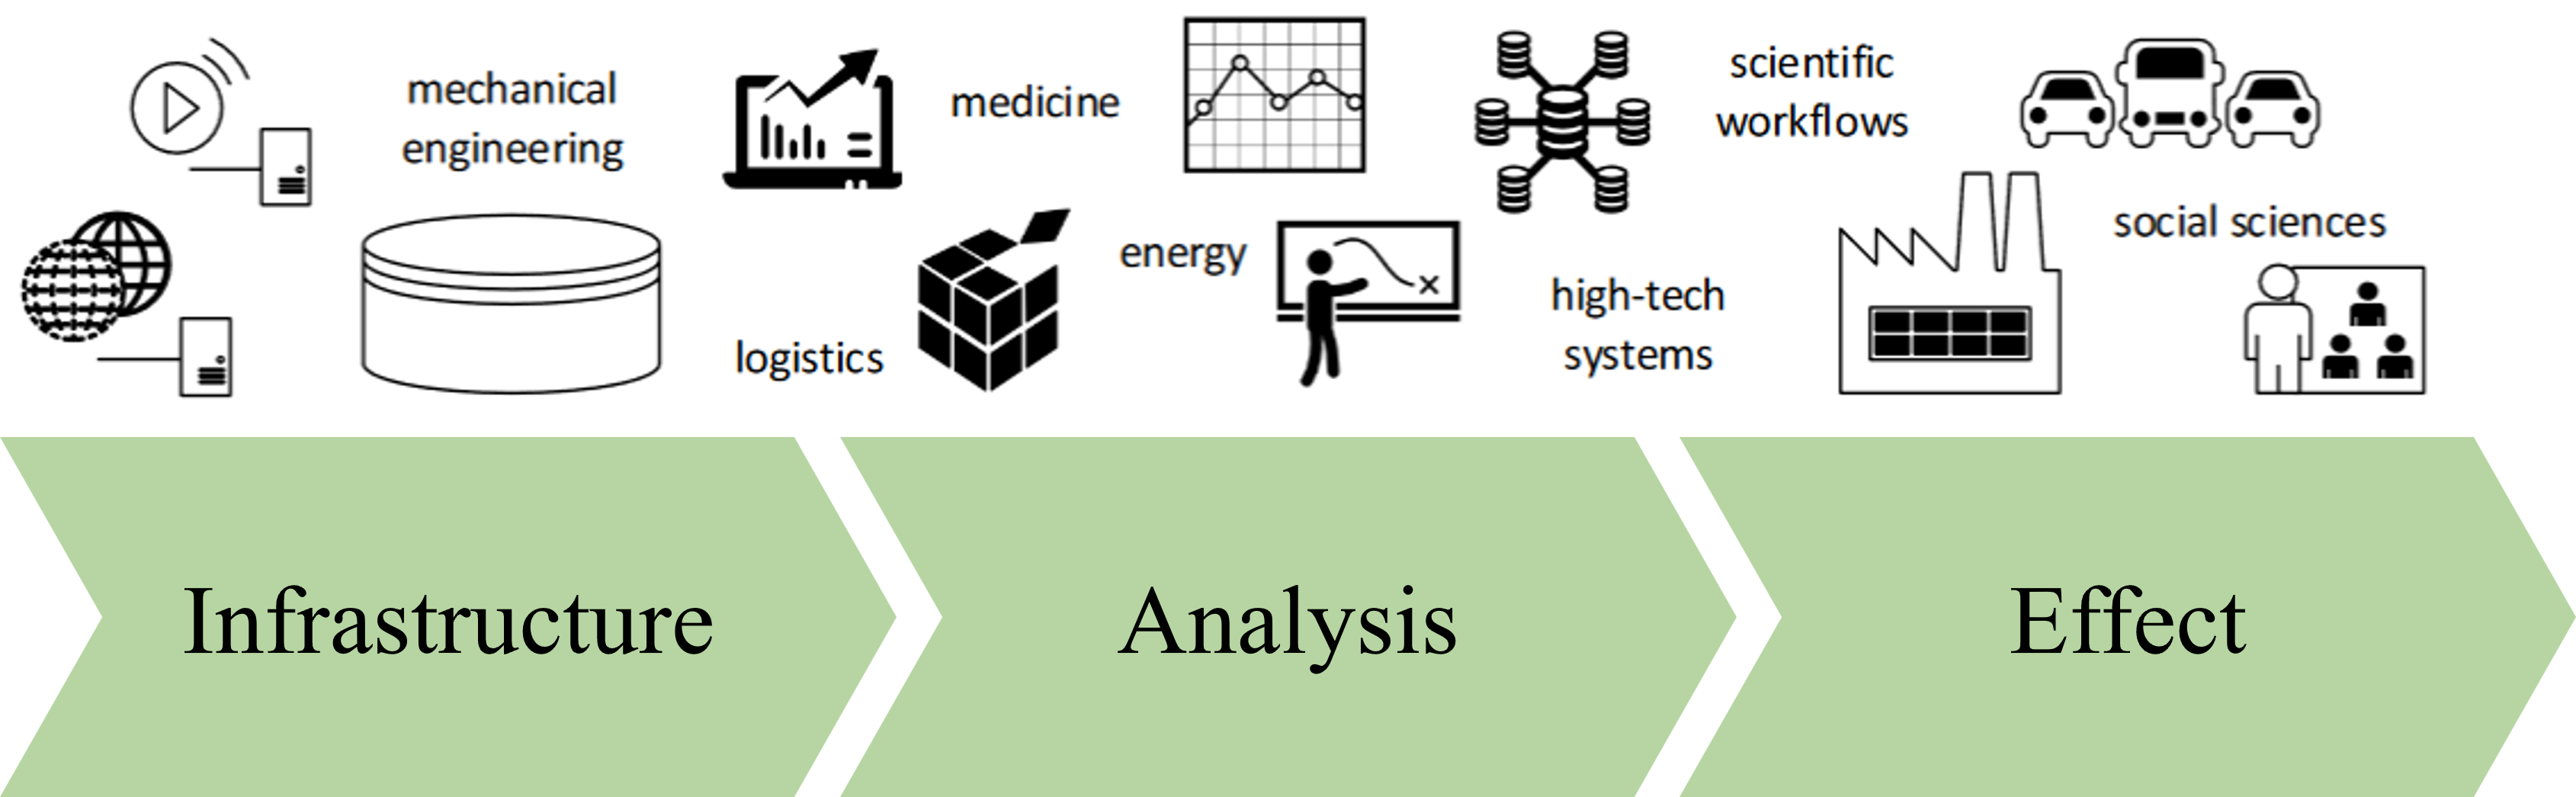
\includegraphics[width=0.75\textwidth]{assets/basics/pipeline.png}
  \caption{Pipeline of data science}
  \label{fig:1_pipeline}
\end{figure}

Let's look at the individual components. The first step to pay attention to when wanting to handle data is the \sidenote{Infrastructure}\textbf{infrastructure} with the keywords \textbf{"volume and velocity"}. The main challenge is making things scalable and instant (responsiveness). Important terms are for example:
\begin{itemize}
  \item Instrumentation
  \item Big data infrastructures, distributed systems
  \item Data engineering (databases and data management)
  \item Programming
  \item Security
\end{itemize}

Next, we have the step of the actual \sidenote{Analysis}\textbf{analysis} concerned with \textbf{extracting knowledge} from data. The core challenge can be put as providing answers to known and unknown unknowns. Important terms are for example:
\begin{itemize}
  \item Statistics, algorithms
  \item Data and process mining
  \item Machine learning, artificial intelligence
  \item Operations research
  \item Visualization
\end{itemize}

Finally, we also need to be concerned with the \sidenote{Effects}\textbf{effect} of our results on people, organizations, and society. The main challenge of this pipeline step is to do \textbf{responsibly} perform data handling. Important terms are for example:
\begin{itemize}
  \item Ethics and privacy, and IT law
  \item Human-technology interaction
  \item Operations management
  \item Business models, entrepreneurship
\end{itemize}

This course will look into all the steps of the pipeline, but the main focus lies on the data analysis.


\subsection*{Four generic data science questions}
Important to answering all these questions is to keep attention to all three pipeline steps, so not only what analysis we need to perform to answer them, but also how we collect our input (data) and how to deal with our output (result).

Nonetheless, here are the four generic data science questions, with variety in terms of difficulty and predicting the future:
\begin{enumerate}
  \item \textbf{What} happened?
  \item \textbf{Why} did it happen?
  \item What will happen in the \textbf{future}?
  \item What is the \textbf{best} that can happen?
\end{enumerate}


\subsection{Types of data}
Now that we know that we have some kind of data as our input, we need to take a look at what this data can look like. Generally speaking, there are two types:
\begin{itemize}
  \item \sidenote{Structured data}Structured data like age, time, gender, class, etc., and
  \item \sidenote{Unstructured data}Unstructured data like text, audio, video, etc.
\end{itemize}

For \textbf{structured data} we have a further subdivision into structured data types. The data types depicted in \ref{fig:1_structured_data} will be described in detail.

\begin{figure}[H]
  \centering
  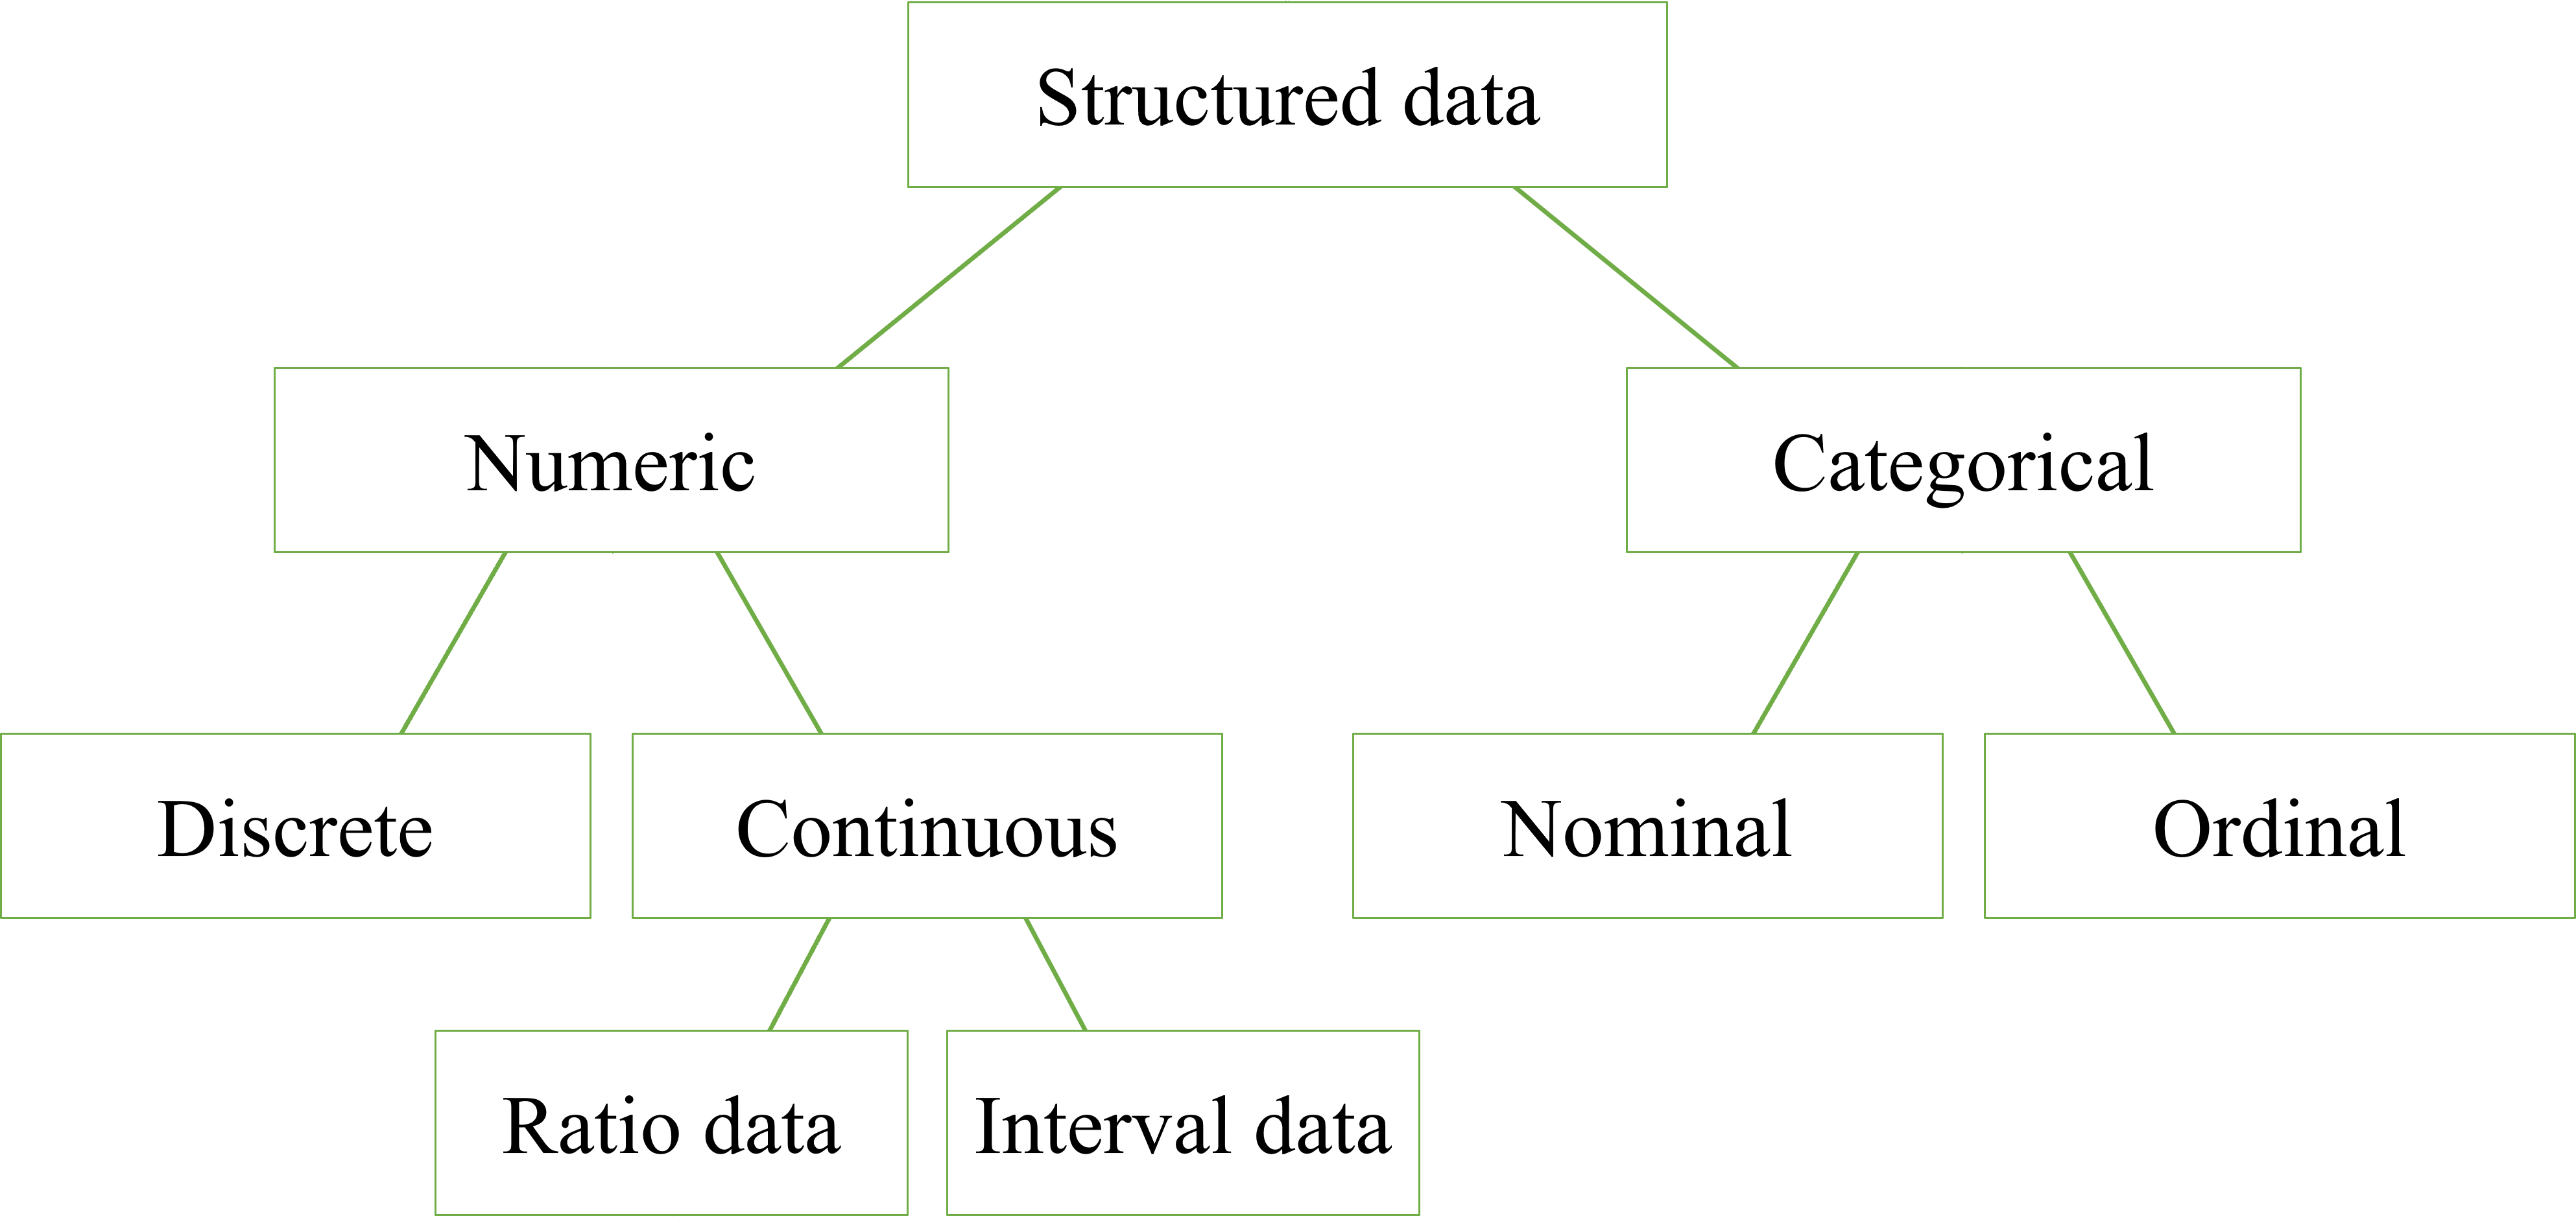
\includegraphics[width=0.6\textwidth]{assets/basics/structured_data.png}
  \caption{Overview structured data types}
  \label{fig:1_structured_data}
\end{figure}

\begin{itemize}
  \item \sidenote{Categorical data}\textbf{Categorical} data can be stored and identified based on names or labels given to them and is also known as "qualitative" data. Matching can be applied, where data is grouped based on similarities.
  
  \item Concretely, \sidenote{Nominal data}\textbf{nominal} data or naming data has a label and its characteristic similar to a noun and doesn't imply an order. {\footnotesize\color{ForestGreen}(Example: name, color=red, country=NL)}
  
  \item \sidenote{Ordinal data}\textbf{Ordinal} data on the other hand is ranked, ordered, or used on a rating scale. This means, you can count and order ordinal data but are not able to measure it. {\footnotesize\color{ForestGreen}(Example: risk=medium, score=good)}
  
  \item In contrast to categorical data, we also have \sidenote{Numerical data}\textbf{numerical} data referring to data in the form of numbers instead of another language or descriptive form. It is also known as "quantitative" data. Important is the ability to be statistically and arithmetically calculated (allowing for $+, -, >, =, \dots$).
  
  \item One subtype of numerical data is \sidenote{Discrete data}\textbf{discrete} data representing countable items, that are collected in a list (finite or infinite). {\footnotesize\color{ForestGreen}(Example: number of items=5, age=18)}
  
  \item Then, there's also \sidenote{Continuous data}\textbf{continuous} data in the form of intervals or ranges. The data represents measurements with their intervals falling on a number line (so counting isn't involved).
  
  \item Continuous data can now be further distinguished. One subtype is \sidenote{Interval data}\textbf{interval} data where the data can be measured only along a scale at equal distances from each other, so only addition and subtraction operations are allowed. There is no true zero (and hence no $\cdot, /$). {\footnotesize\color{ForestGreen}(Example: data=11-11-2018, temp=18.5°C)}
  
  \item And finally, we have \sidenote{Ratio data}\textbf{ratio} data describing measurement with a defined (true) zero point. {\footnotesize\color{ForestGreen}(Example: dropout=33\%, speed=128.34km/h)}
\end{itemize}

For \textbf{unstructured data}, we just take the raw data and interpret it as a stream of bits. This goes for text, audio, images, signals, and videos exactly the same. Examples can be seen in \ref{fig:1_unstructured_data}.

\begin{figure}[H]
  \centering
  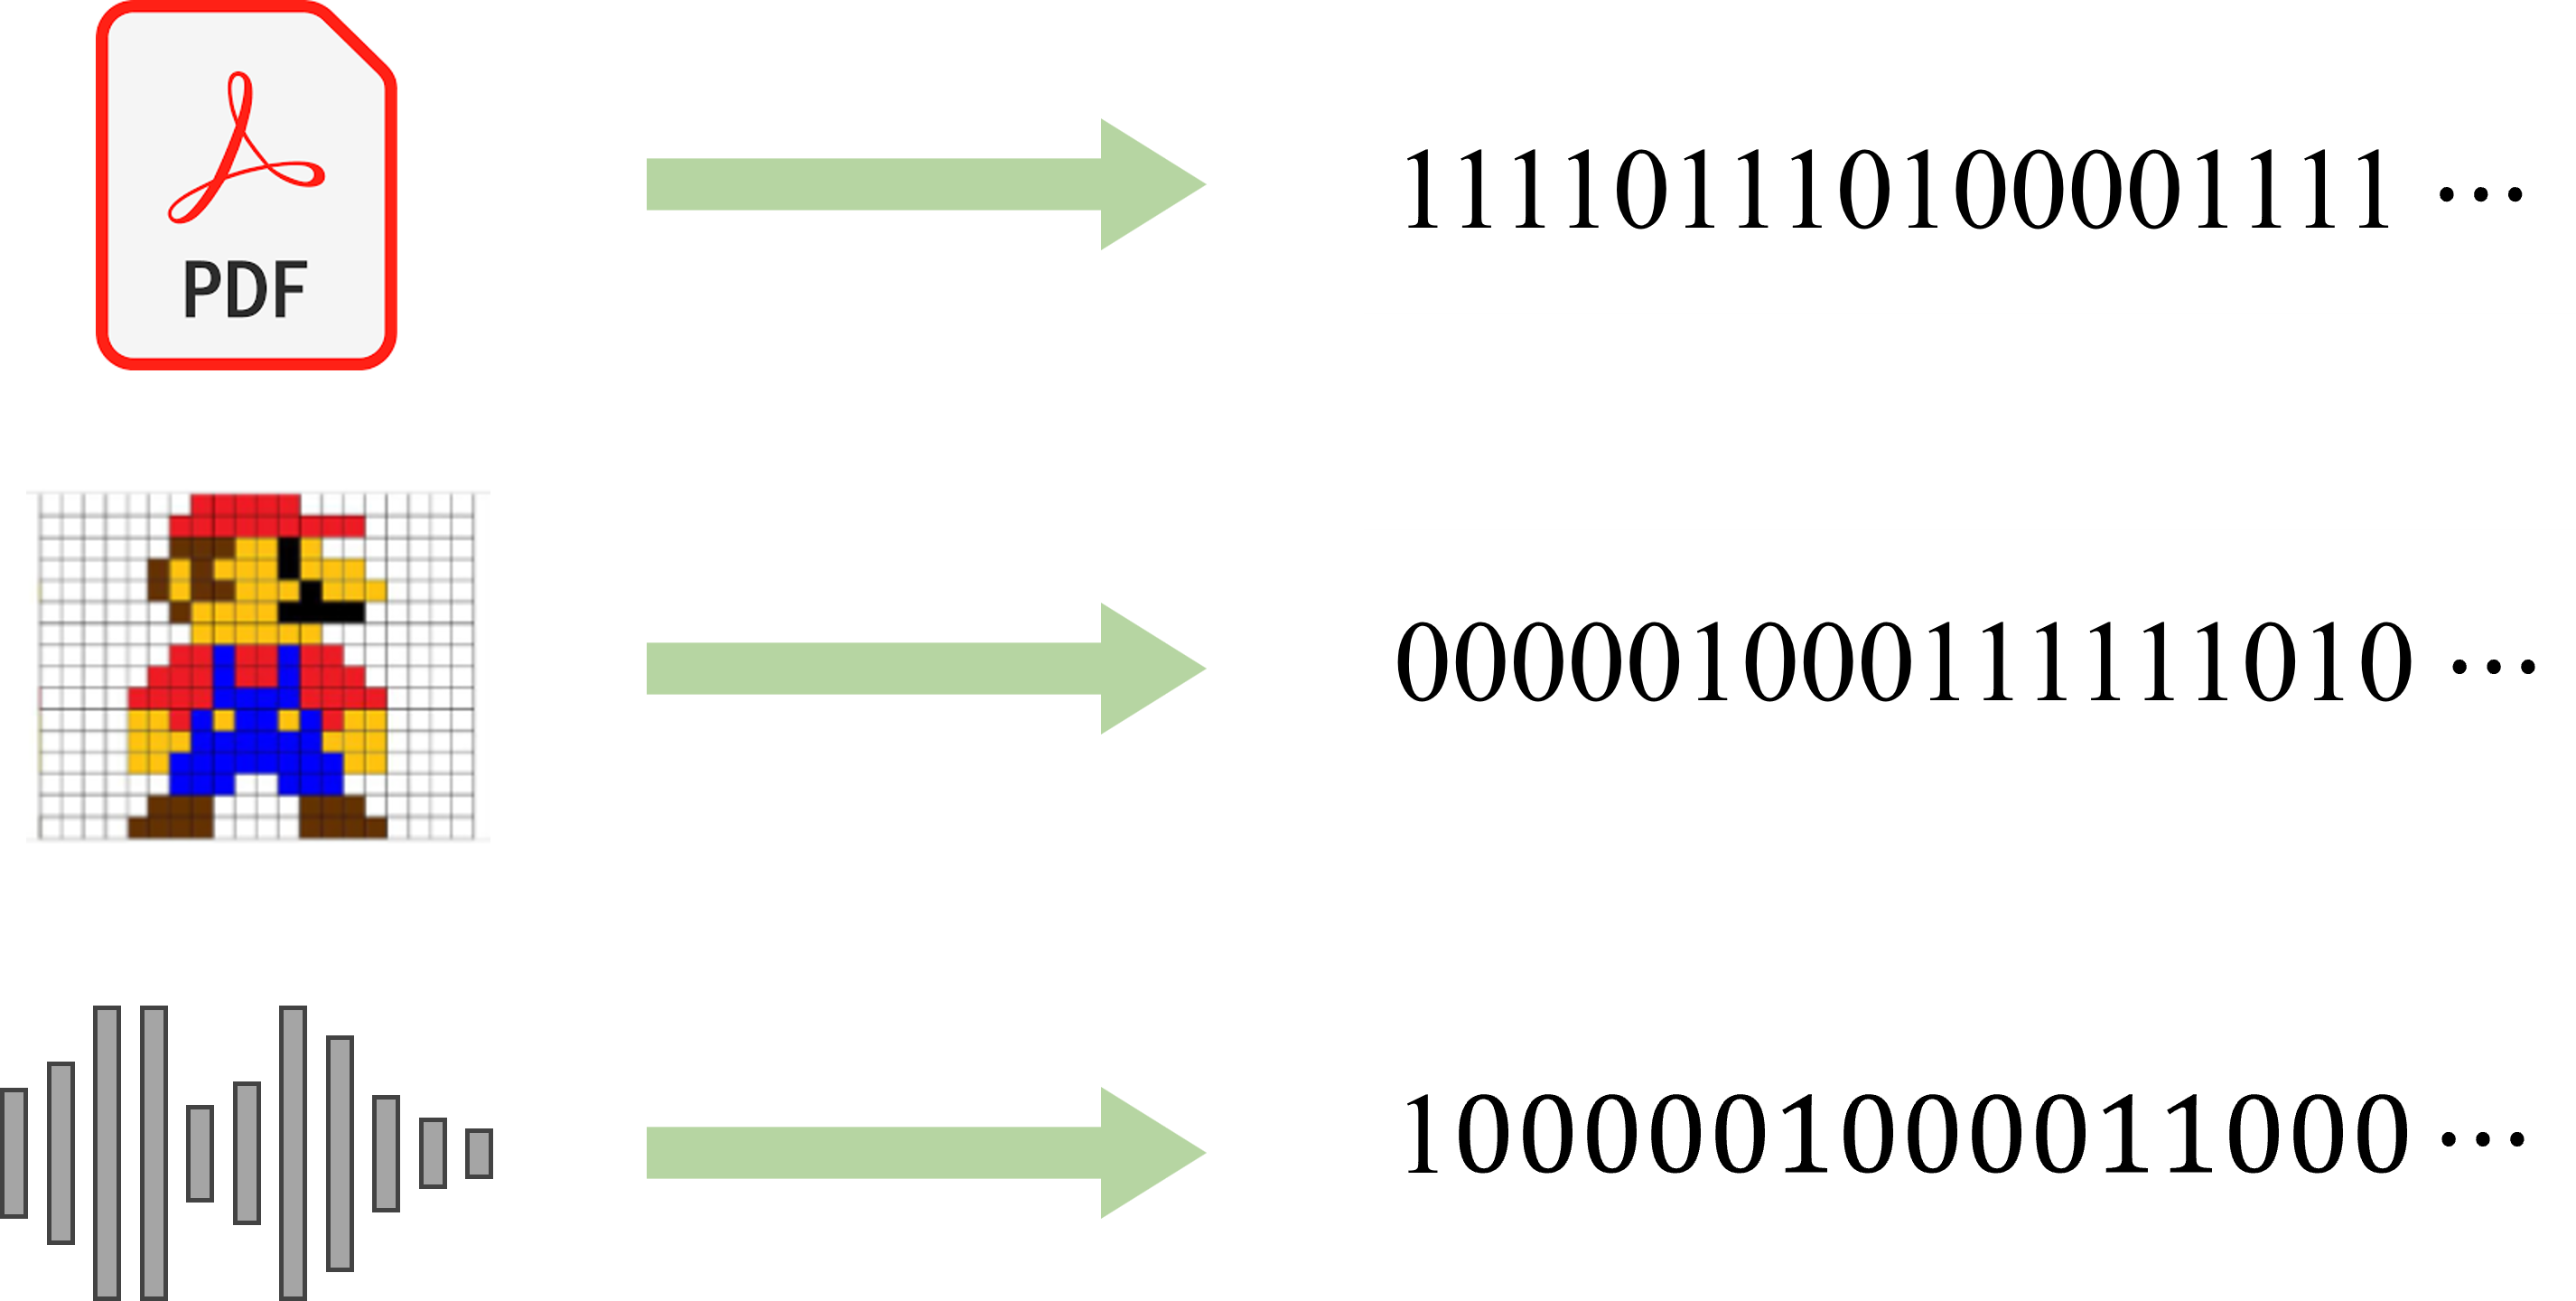
\includegraphics[width=0.4\textwidth]{assets/basics/unstructured_data.png}
  \caption{Input for unstructured data}
  \label{fig:1_unstructured_data}
\end{figure}

Data can now be stored and ordered together by putting it into \sidenote{Tabular data}\textbf{tables}. Concretely, columns represent different features (can be different kinds of data types) whereas rows describe data instances (also known as individuals, entities, cases, objects, or records). Examples can be seen in \ref{fig:1_table_data}.

\begin{figure}[H]
  \centering
  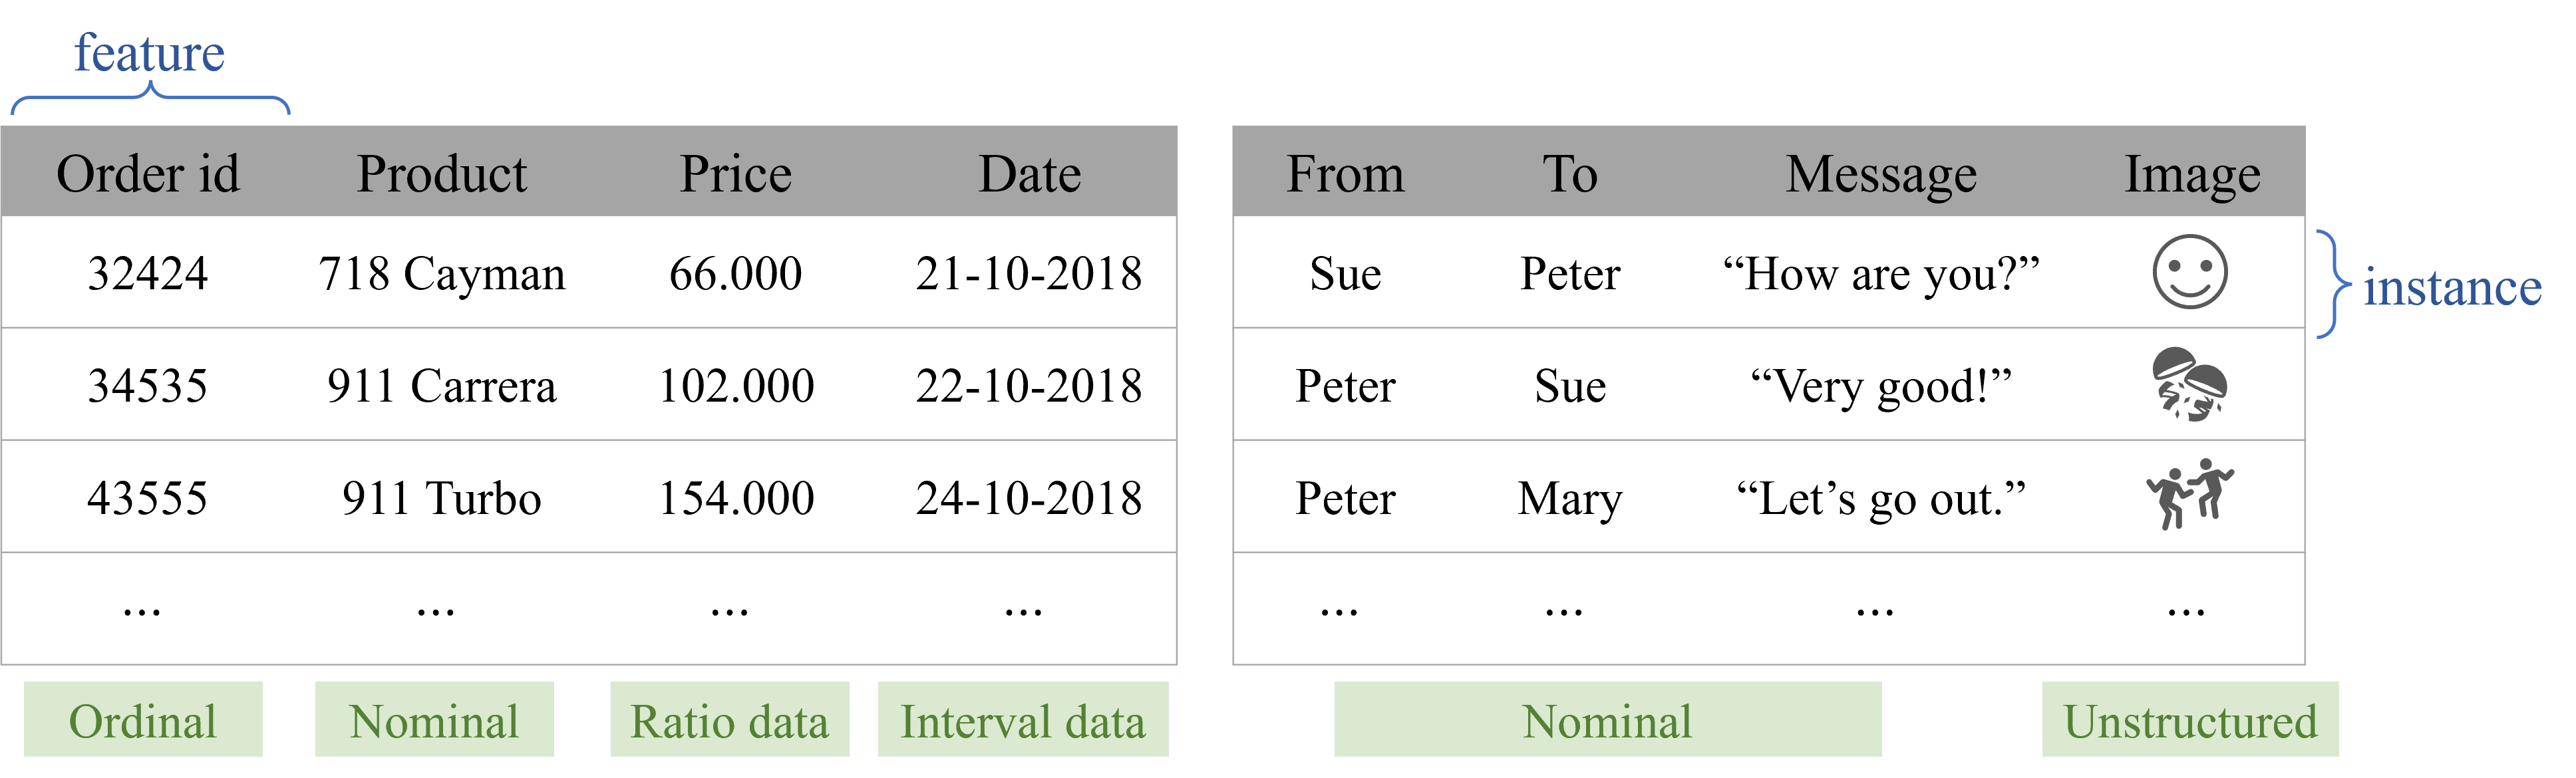
\includegraphics[width=0.9\textwidth]{assets/basics/table_data.png}
  \caption{Table data with data types}
  \label{fig:1_table_data}
\end{figure}

Features \sidenote{Features} can now be raw or derived (e.g. max, min, average, rank, bin, $\dots$). An important aspect is time, as it cannot decrease and we usually want to predict the future based on the past. 

An important distinction to be made when it comes to tabular data is whether the items are labeled or not.
\begin{itemize}
  \item \sidenote{Labelled data}In case of labelled data we have \textbf{descriptive features} and a \textbf{target feature}.
  \begin{itemize}
    \item The \sidenote{Descriptive features}descriptive features are also known as predictor variables or independent variables.
    \item Alternative names for \sidenote{Target feature}target features are response variable, dependent variable, or also label.
  \end{itemize}
  \item \sidenote{Unlabelled data}Unlabelled data on the other hand doesn't have a selected target feature.
\end{itemize}
\subsection{Supervised and unsupervised learning}
Derived from the different kinds of tabular data, we have two fundamental learning paradigms. Exemplary input data and possible results for both paradigms can be seen in \ref{fig:1_sv_vs_usv}.

\begin{figure}[h]
  \centering
  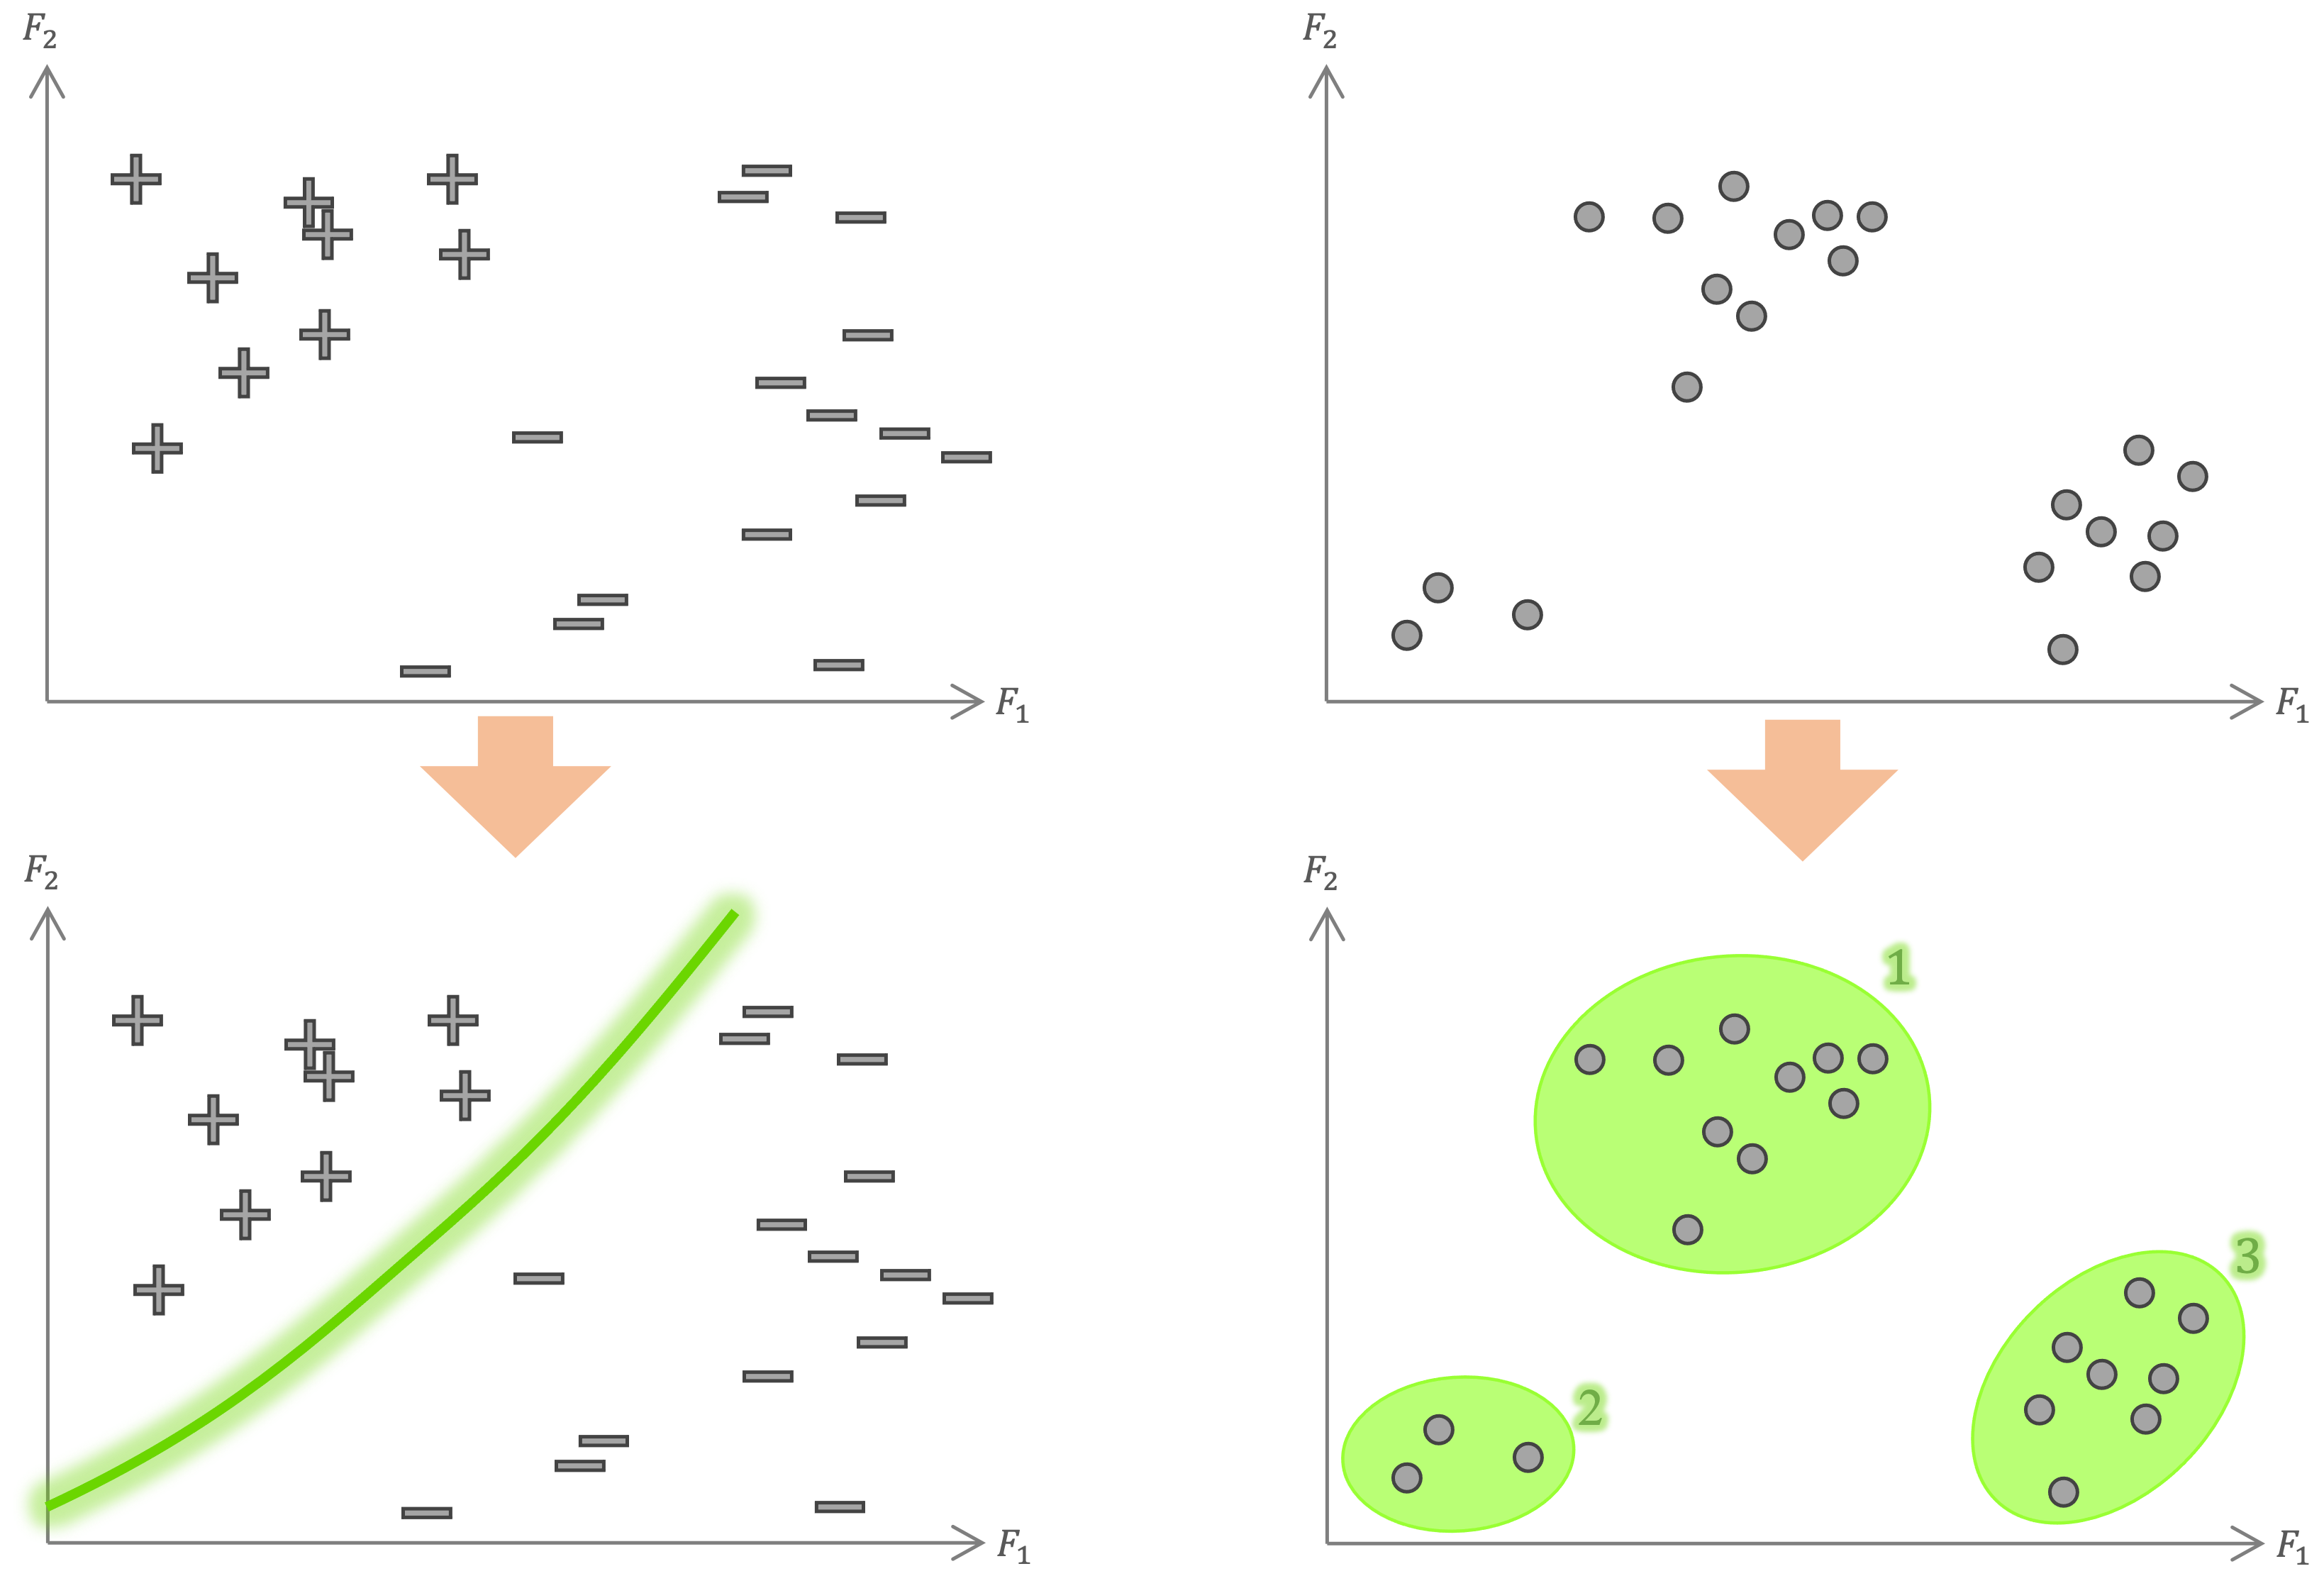
\includegraphics[width=0.6\textwidth]{assets/basics/SV_vs_US.png}
  \caption{Comparing supervised (left) and unsupervised (right) learning}
  \label{fig:1_sv_vs_usv}
\end{figure}

In the case of labeled data, we can apply \textbf{supervised learning}\sidenote{Supervised learning}. The goal is to find a "rule" in terms of descriptive features explaining the target feature as well as possible. \begin{note}Examples include:
\begin{itemize}
  \item Hospital environments where the target variable can be "recover" (yes or no), and the descriptive variables can be age, gender, smoking, $\dots$.
  \item University environments where the target variable can be "drops out" (yes or no), and the descriptive variables can be {\color{ForestGreen}mentor, prior education, $\dots$}.
  \item Production environments where the target variable can be "order is delivered in time" (yes or no), and the descriptive variables can be product, agent, $\dots$.
\end{itemize}\end{note}

In contrast to labeled data, we can also have instances without target labels, where we can only apply techniques of \textbf{unsupervised learning}\sidenote{Unsupervised learning}. The goal is to find clusters or patterns.
\begin{itemize}
  \item \textbf{Clusters}\sidenote{Cluster} are homogeneous sets of instances. \begin{note}Examples include finding similar groups of patients, students, customers, orders, cars, companies, and so on.\end{note}
  \item \textbf{Patterns}\sidenote{Pattern} on the other hand reveal hidden structures in the data, so basically the unknown unknowns. Rules of some form can be found in many environments. \begin{note}Examples can look like:
  \begin{itemize}
    \item Customers who buy bread and butter typically pay by phone.
    \item Patients who drink and smoke typically pay the hospital bill earlier than others.
    \item Products produced by team A on Monday tend to be returned more frequently by customers.
  \end{itemize}\end{note}
\end{itemize}

Interesting to regard is process discovery as a form of unsupervised learning in the way that a process model is just a very sophisticated rule. Important to mention, that this task can get very complex very quickly.



\subsection*{Terminology}
Important to see for all of data science: many different names are used to refer to the key disciplines contributing to data science.
\begin{itemize}
  \item This includes statistics, data analytics, data mining, machine learning, artificial intelligence, predictive analytics, process mining, generative AI, etc.
  \item Since frequently the same name is used for different concepts (names describe heavily overlapping areas), they really need to be put in context and interpreted accordingly.
\end{itemize}

The point can be highlighted when looking at scoping machine learning. Here are examples of confusions:
\begin{itemize}
  \item Sometimes "machine learning" is used as a synonym for "deep neural networks" and sometimes they cover the entire spectrum of learning techniques.
  \item Neural networks can be used as classifiers. But this doesn't imply that numerous classification techniques developed in data mining are part of machine learning in the narrow sense.
\end{itemize}
How confusing specifically the arrangement of terms around machine learning is and how fluent and unclear the actual terms are, is depicted in \ref{fig:1_ml_terminology}.

\begin{figure}[H]
  \centering
  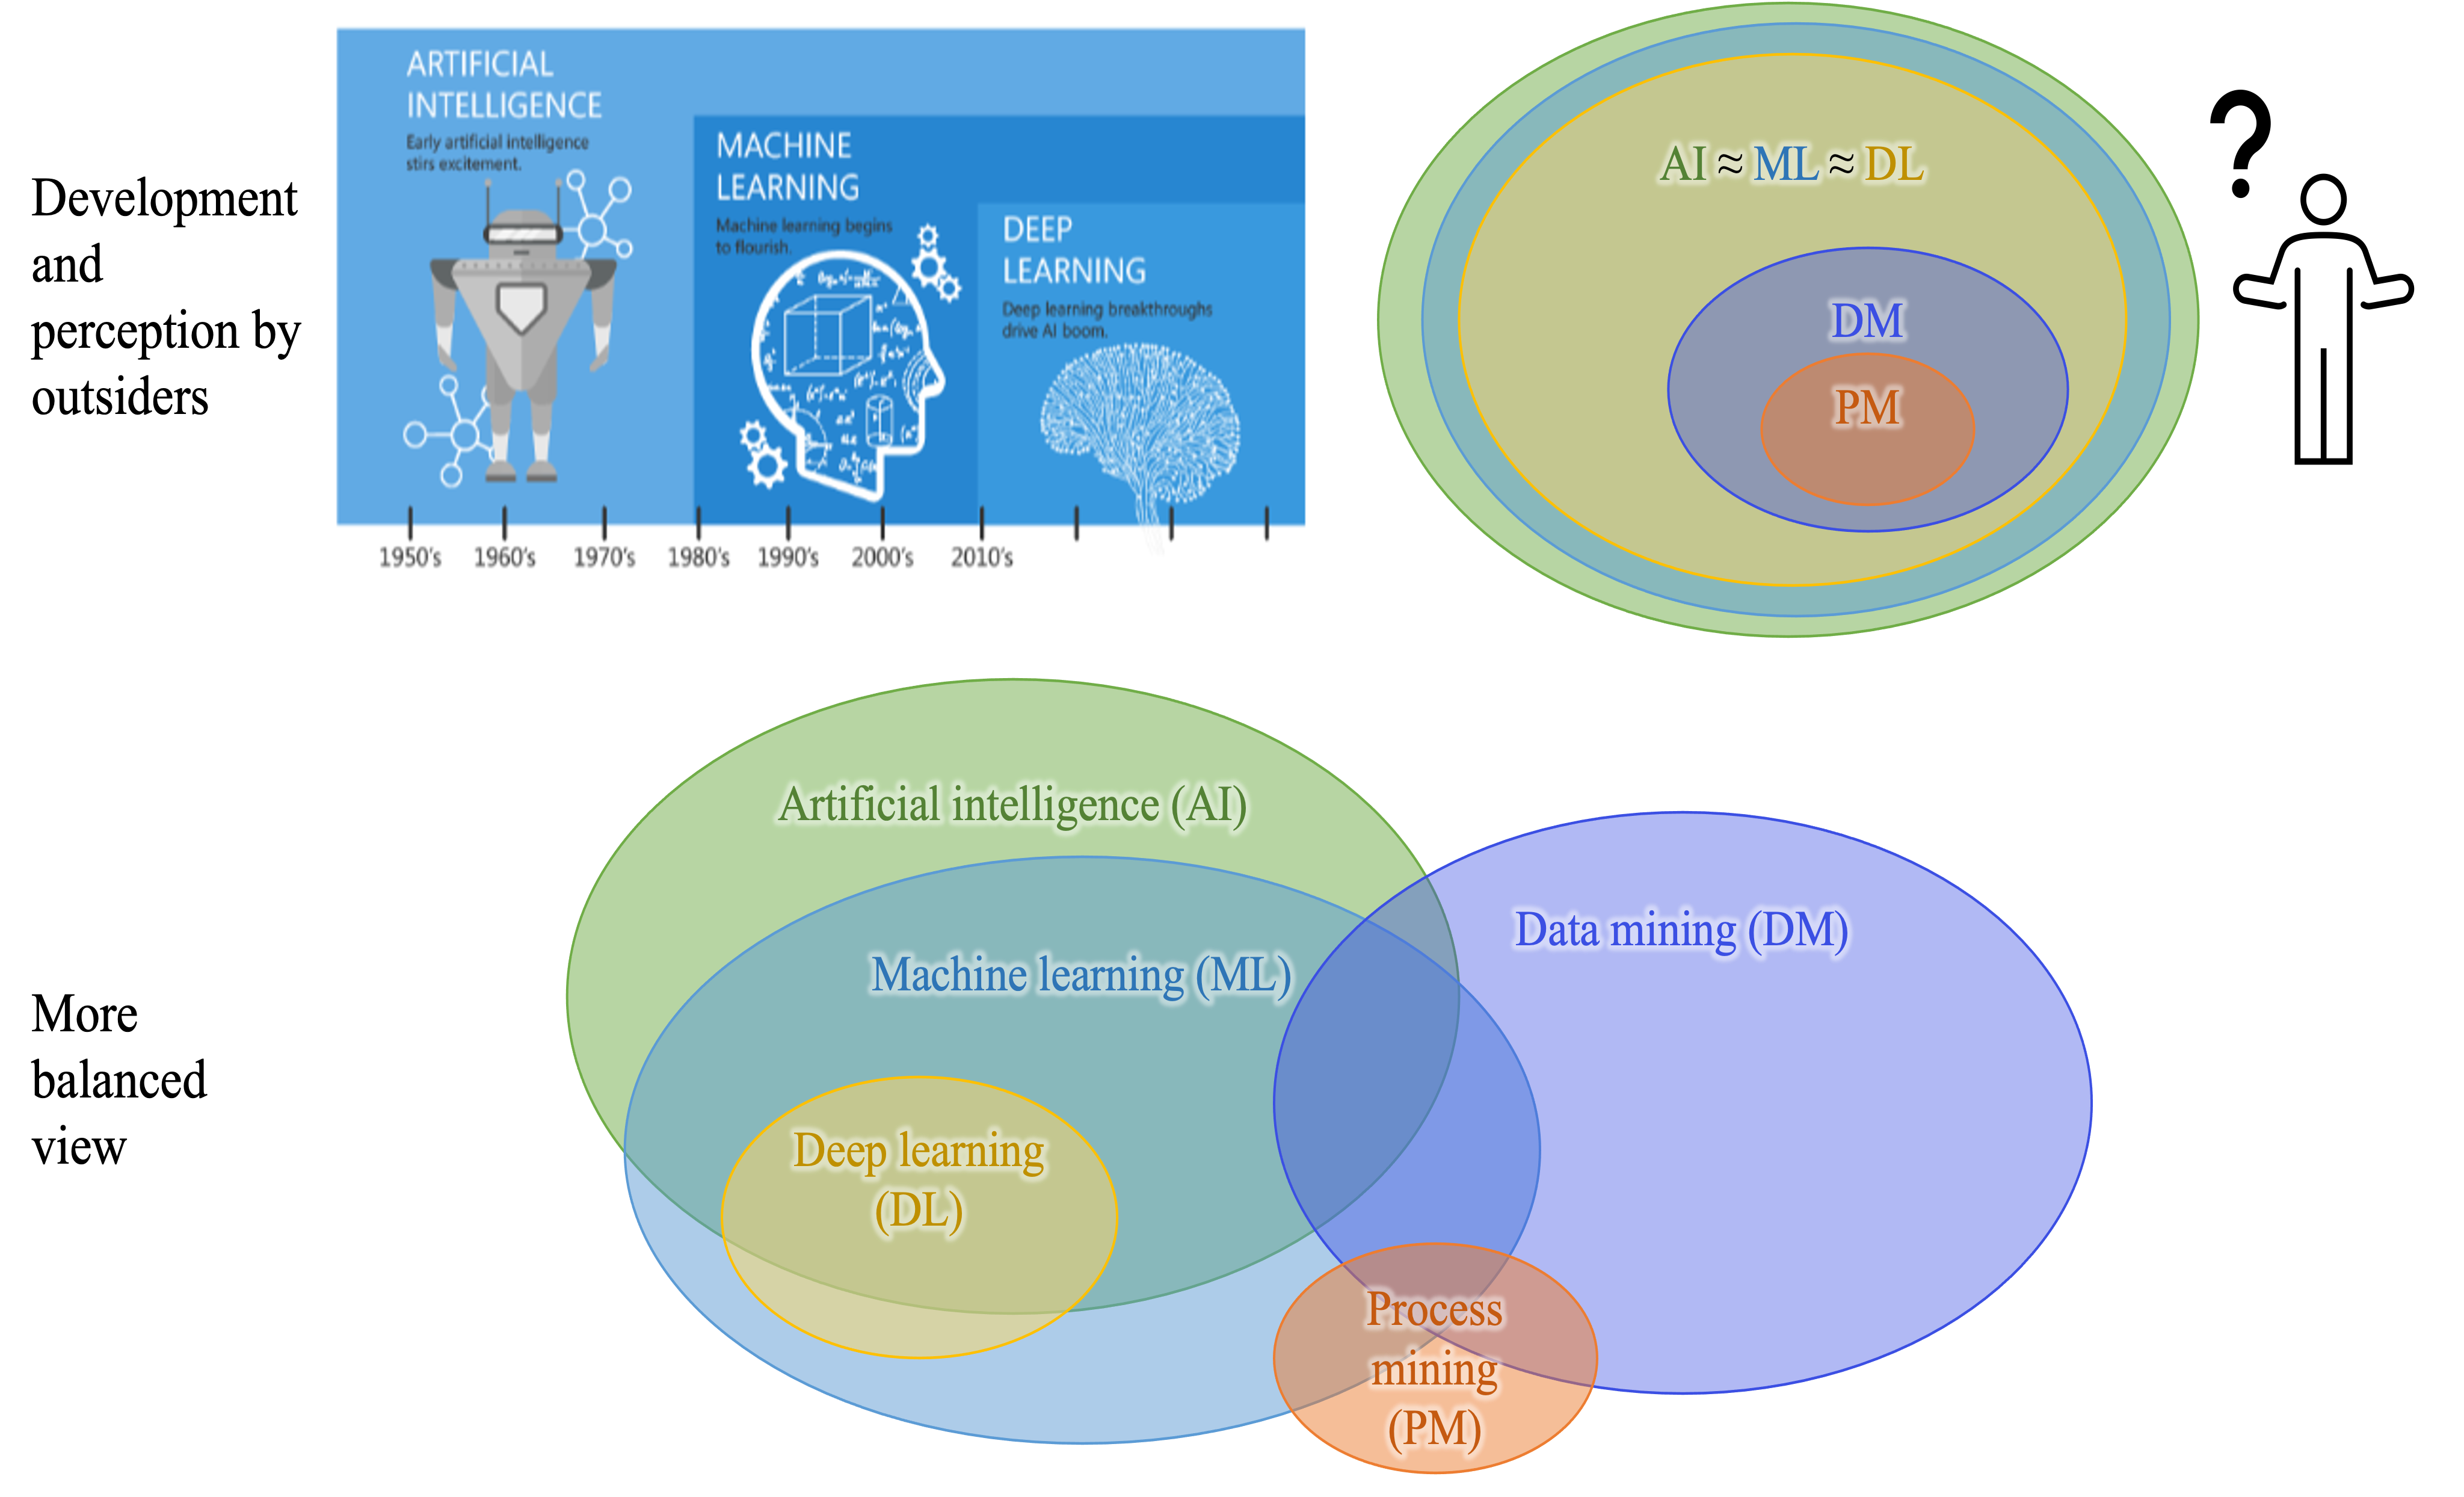
\includegraphics[width=0.7\textwidth]{assets/basics/confusion_terminology.png}
  \caption{Terms around machine learning}
  \label{fig:1_ml_terminology}
\end{figure}



\subsection{Data science process}
There are many different lifecycle models to describe phases in a data science project. This section will give a quick overview of some important ones.

We'll start with \textbf{CRISP-DM}\sidenote{CRISP-DM} which stands for "Cross-industry standard process for data mining". It was developed in the late 1990s by different involved companies (SPSS, Teradata, Daimler AG, NCR Corporation, Ohra). The process consists of multiple steps playing together as visualized in \ref{fig:1_crisp_dm}

\begin{figure}[H]
  \centering
  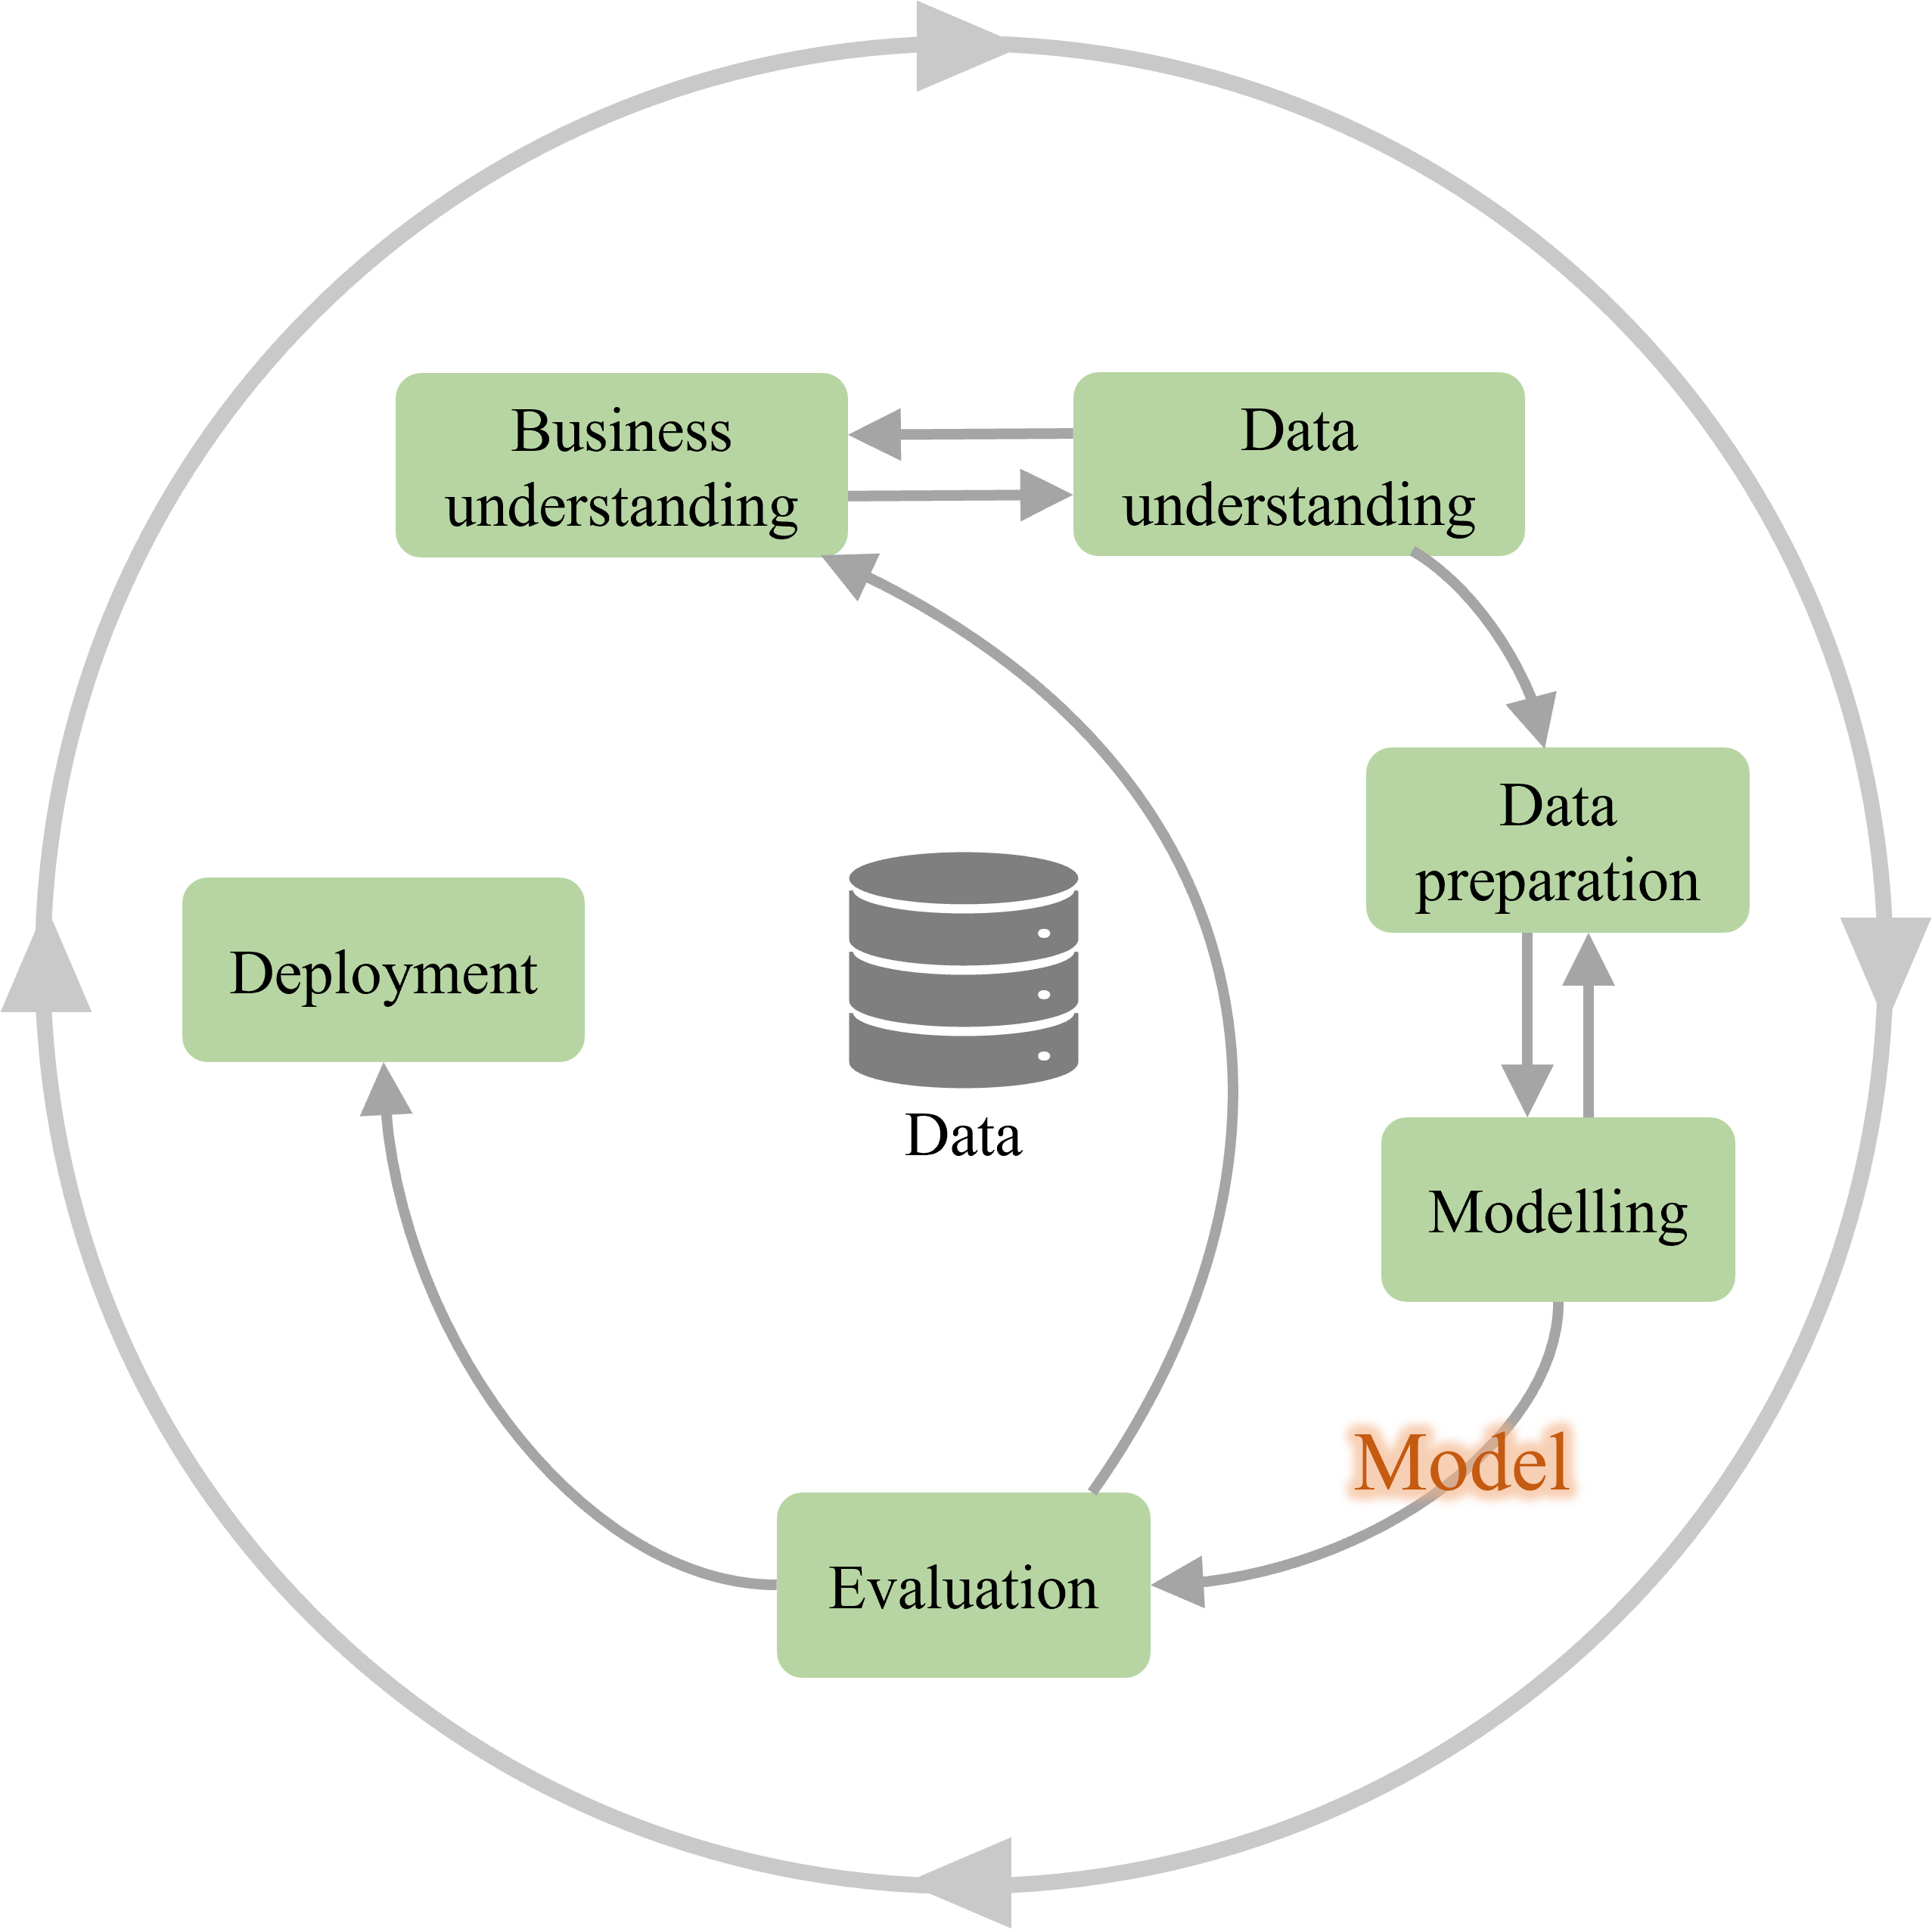
\includegraphics[width=0.5\textwidth]{assets/basics/crisp-dm.png}
  \caption{CRISP-DM process}
  \label{fig:1_crisp_dm}
\end{figure}

\begin{longtable}{p{0.0025\linewidth} >{\color{black}}p{0.35\linewidth} >{\color{gray}\footnotesize}p{0.6475\linewidth}}
  \multicolumn{3}{l}{\textbf{Business understanding}} \\
  & Determine business objective & Background, business objective, business success criteria \\
  & Situation assessment & Inventory of resources, requirements, assumptions, constraints, risks, contingencies, terminology, costs, benefits \\
  & Determine data mining goal & Data mining goals, data mining success criteria \\
  & Produce project plan & Project plan, initial assessment of tools and techniques \\[5pt]
  
  \multicolumn{3}{l}{\textbf{Data understanding}} \\
  & Collect initial data & Initial data collection report \\
  & Describe and explore data & Data description, exploration report \\
  & Verify data quality & Data quality report \\[5pt]
  
  \multicolumn{3}{l}{\textbf{Data preparation}} \\
  & Starting point: data set & Data set, data set description \\
  & Select data & Rationale for inclusion and exclusion \\
  & Clean data & Data cleaning report \\
  & Construct data & Derived attributes, generated records \\
  & Integrate and format data & Merged/reformatted data \\[5pt]
  
  \multicolumn{3}{l}{\textbf{Modeling}\footnote{The term "modeling" can be misleading, meant is the selection and assumptions (human) or automated learning by a tool or algorithm}} \\
  & Select modeling technique & Modeling technique, modeling assumptions \\
  & Generate test design & Test design \\
  & Build model & Parameter settings, models, model description \\
  & Assess model & Model assessment, revised parameter settings \\[5pt]
  
  \multicolumn{3}{l}{\textbf{Evaluation}} \\
  & Evaluate results & Assessment of data mining results w.r.t. business success criteria, approved models \\
  & Review process & Review of process \\
  & Determine next steps & List of possible actions settings \\[5pt]
  
  \multicolumn{3}{l}{\textbf{Deployment}} \\
  & Plan deployment & Deployment plan \\
  & Plan monitoring and maintenance & Monitoring and maintenance plan \\
  & Produce final report & Final report and final presentation \\
  & Review project & Experience documentation
  
\end{longtable}

Next, we have the \textbf{KDD}\sidenote{KDD} (Knowledge Discovery in Databases) process as shown in \ref{fig:1_kdd}. Another process model also developed by SAS institute is called \textbf{SEMMA}\sidenote{SEMMA} consisting of the phases Sample, Explore, Modify, Model, and Assess.

\begin{figure}[H]
  \centering
  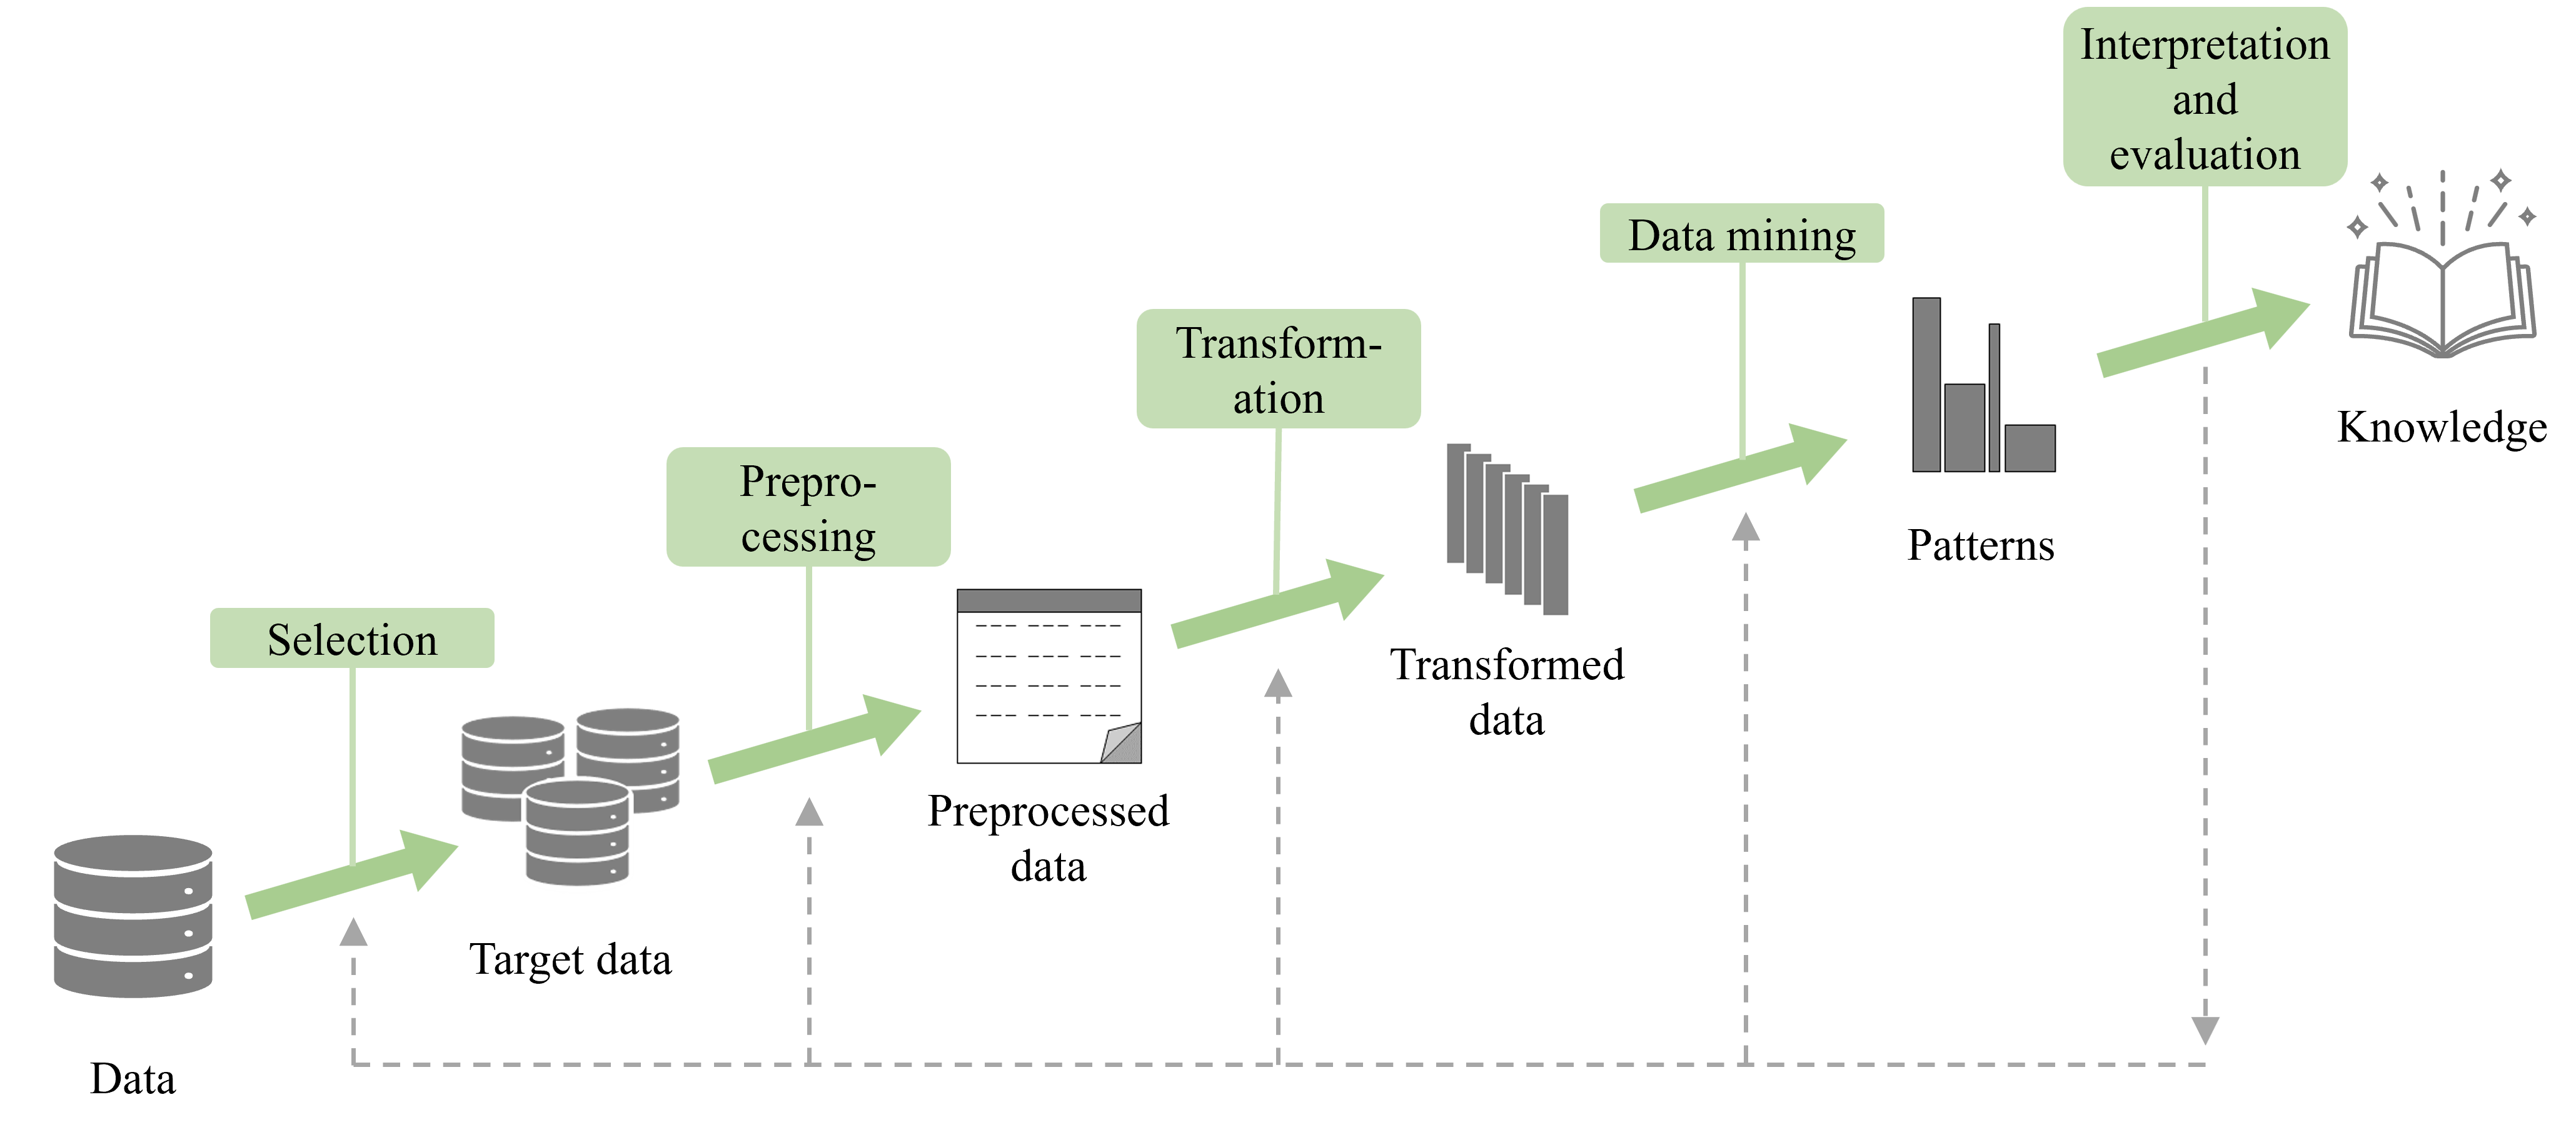
\includegraphics[width=\textwidth]{assets/basics/kdd.png}
  \caption{KDD process}
  \label{fig:1_kdd}
\end{figure}

The next process model is specifically developed for \textbf{L* lifecycle model}\sidenote{L* lifecycle model} with multiple stages as shown in \ref{fig:1_l_star}. 

\begin{figure}[H]
  \centering
  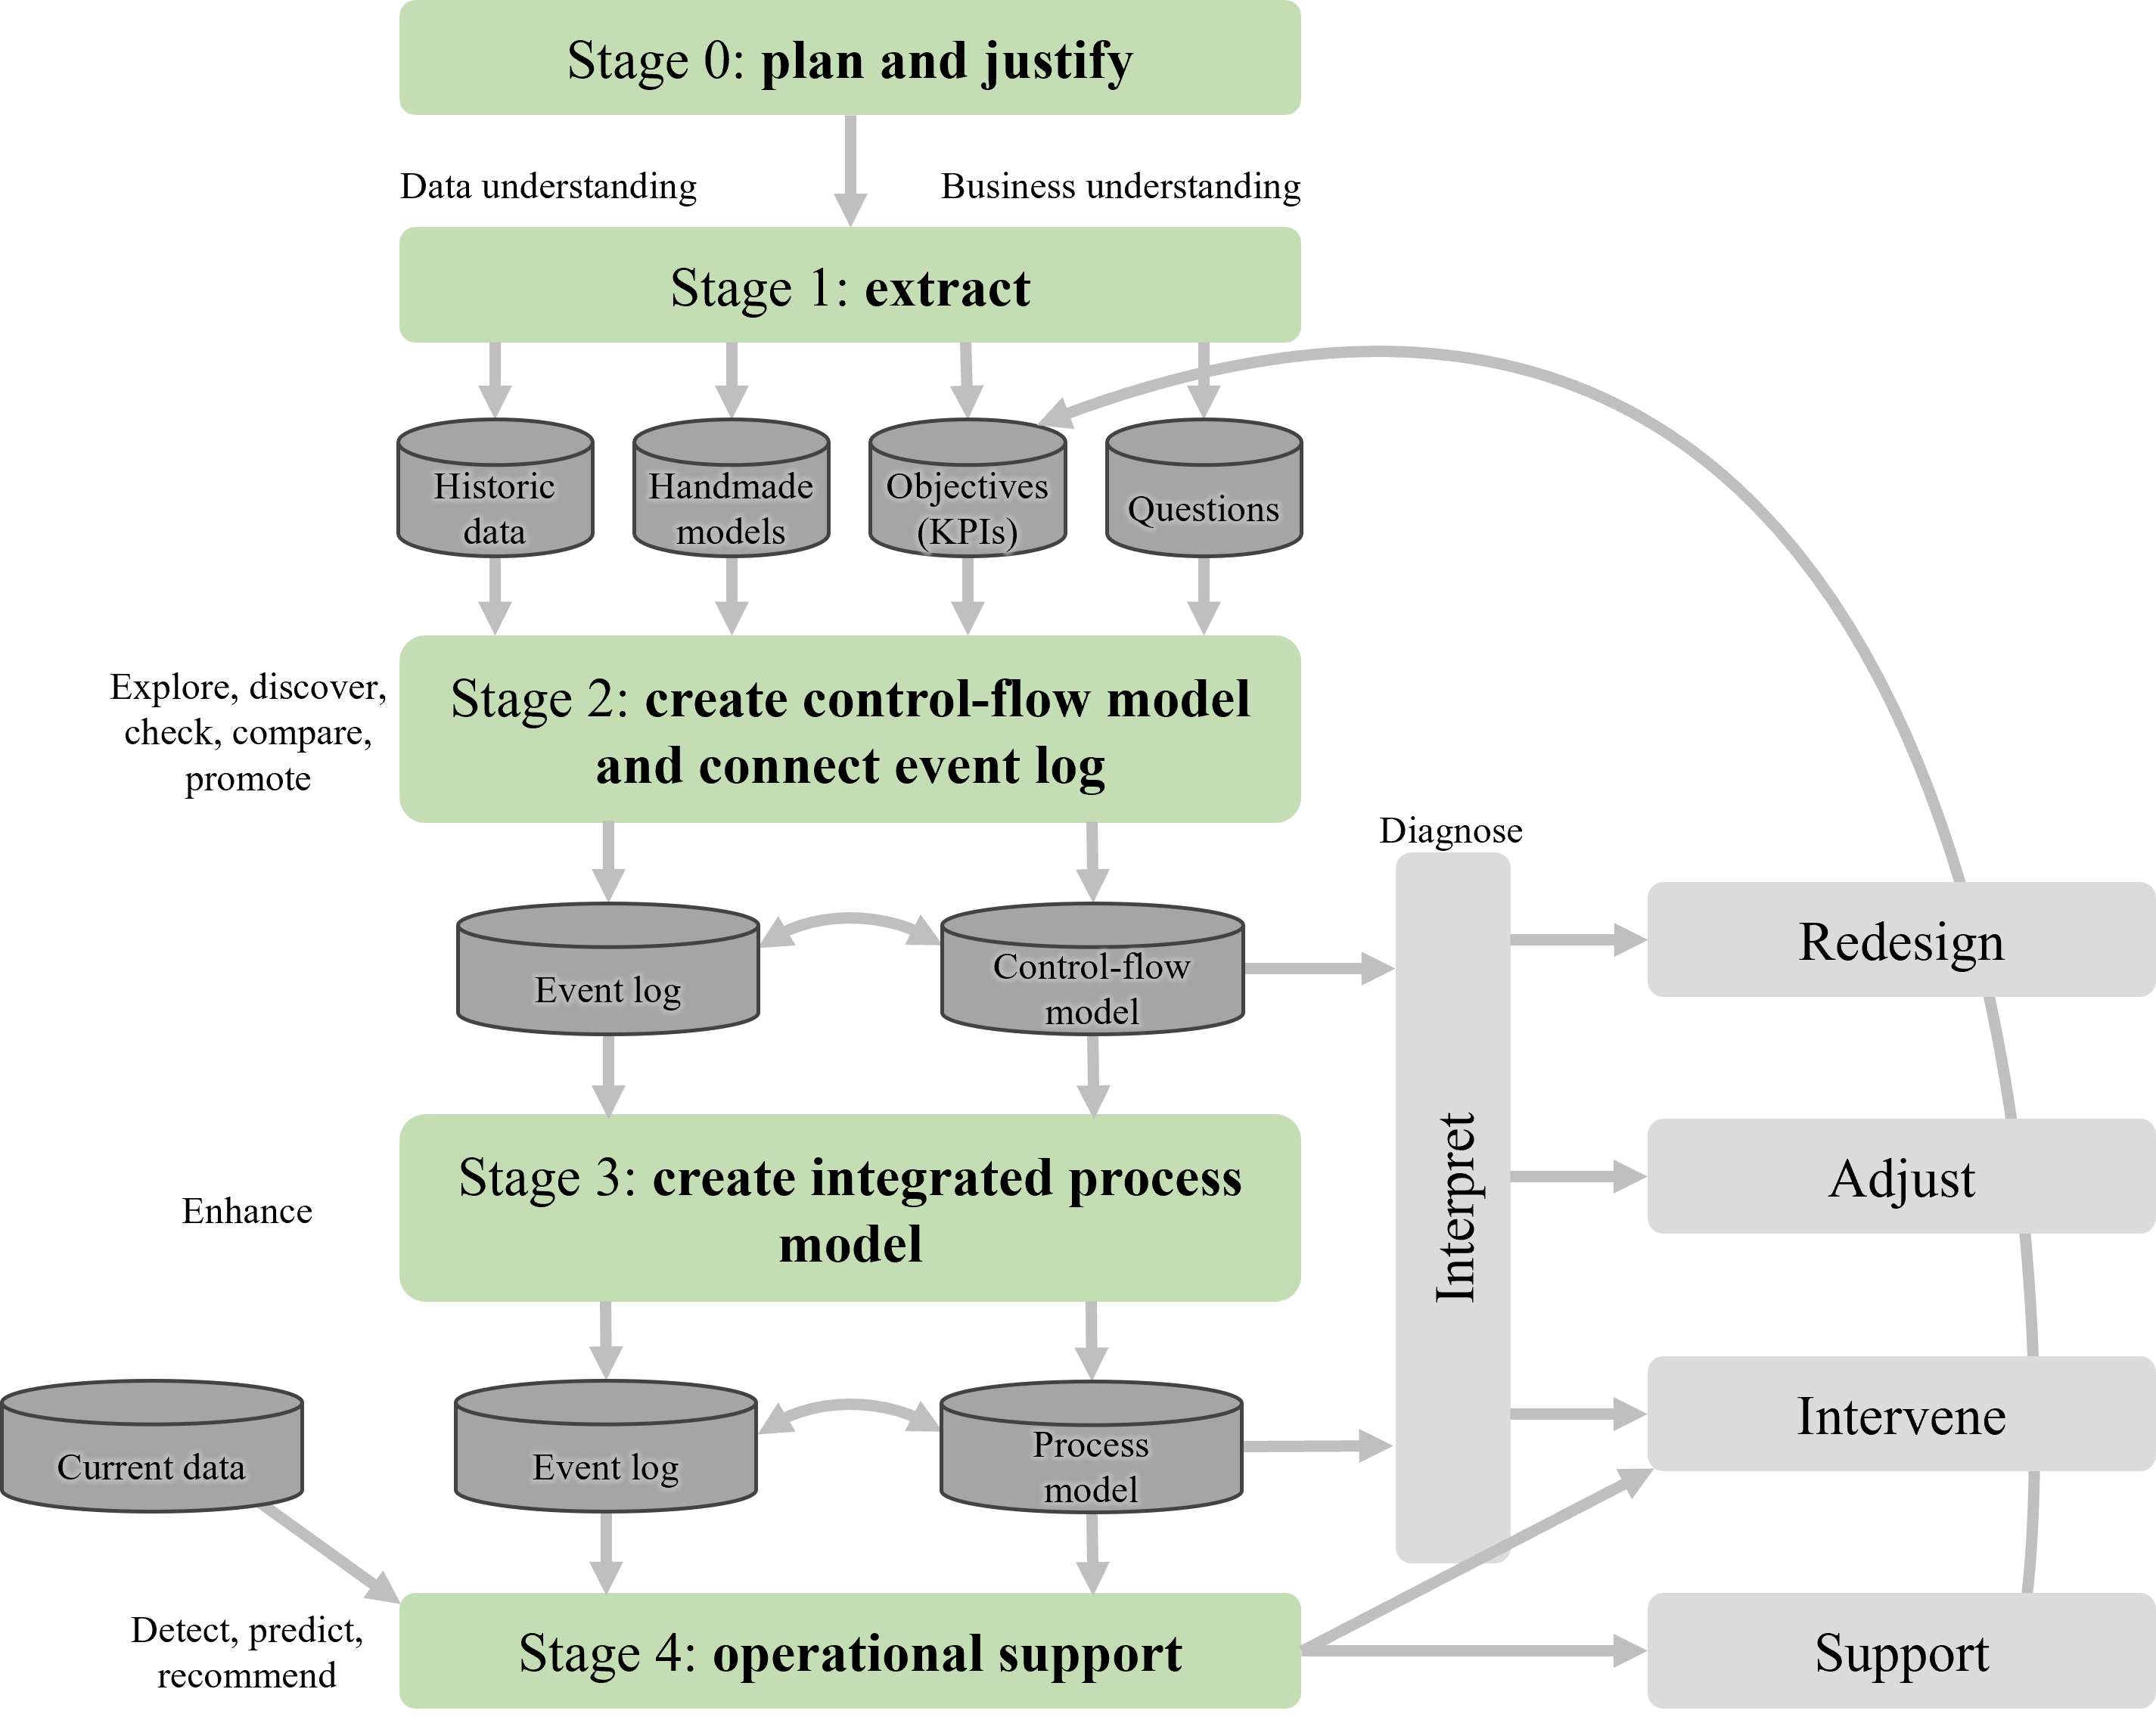
\includegraphics[width=0.7\textwidth]{assets/basics/l_star.png}
  \caption{L* lifecycle model}
  \label{fig:1_l_star}
\end{figure}

Furthermore, we have two methodologies the process model can be related to. Important to implement and solidify are improvements in both.
\begin{itemize}
  \item \textbf{PDCA}\sidenote{PDCA} stands for Plan-Do-Check-Act and is a never-ending cycle with exactly these steps. 
  \item The other one \textbf{DMAIC}\sidenote{DMAIC} stands for Define-Measure-Analyze-Improve-Control, with the following subtasks:
  \begin{itemize}
    \item {\color{gray}\footnotesize Define: launch team, establish charter, plan project, gather VOC/VOB, plan for change}
    \item {\color{gray}\footnotesize Measure: document process, collect baseline data, narrow project focus}
    \item {\color{gray}\footnotesize Analyze: analyze data, identify root causes, identify and remove waste}
    \item {\color{gray}\footnotesize Improve: generate, evaluate, and optimize solutions, pilot, plan and implement}
    \item {\color{gray}\footnotesize Control: control the process, validate project benefits}
  \end{itemize}
\end{itemize}

Finally, we have two processes with the same components, but different ordering of the steps as can be seen in \ref{fig:1_etl_and_elt}. The short terms for the processes are \textbf{ETL}\sidenote{ETL} (extract, transform, load) and \textbf{ELT}\sidenote{ELT} (extract, load, transform).

\begin{figure}[H]
  \centering

  \subcaptionbox{ETL with data warehouse}{
    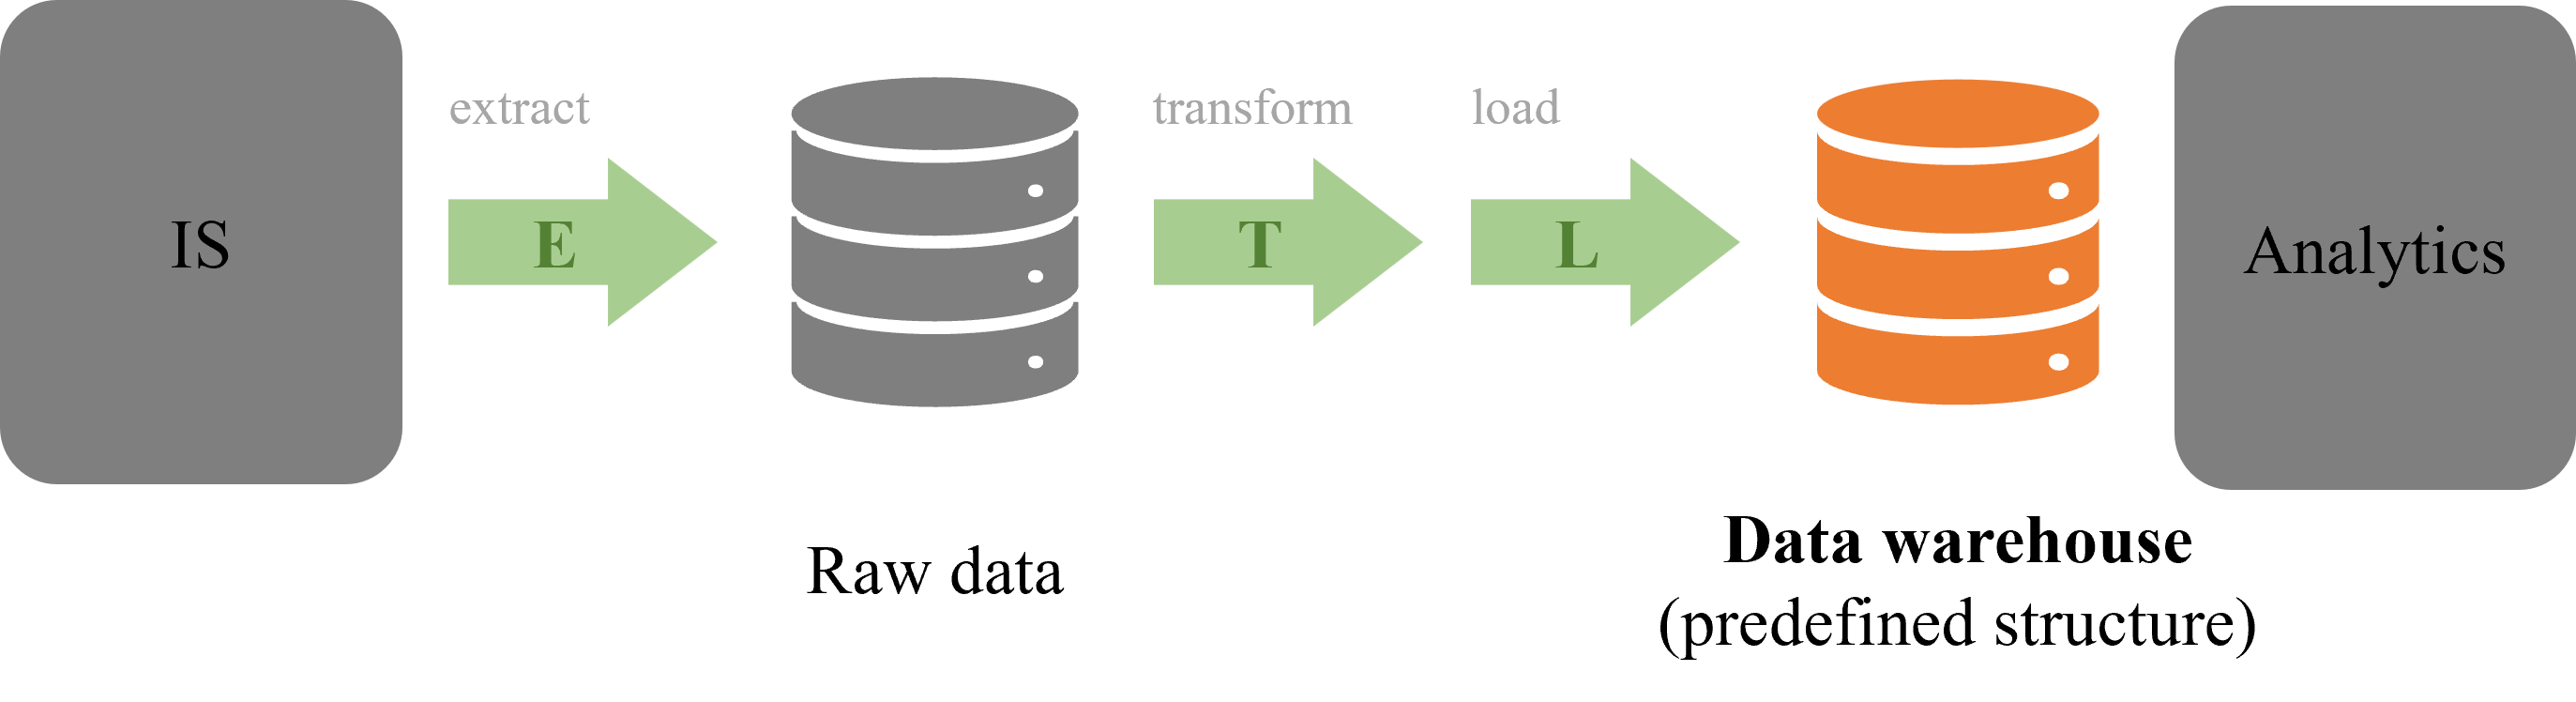
\includegraphics[width=0.45\textwidth]{assets/basics/etl.png}
  }
  \\\vspace*{0.5cm}
  \subcaptionbox{ELT with data lake}{
    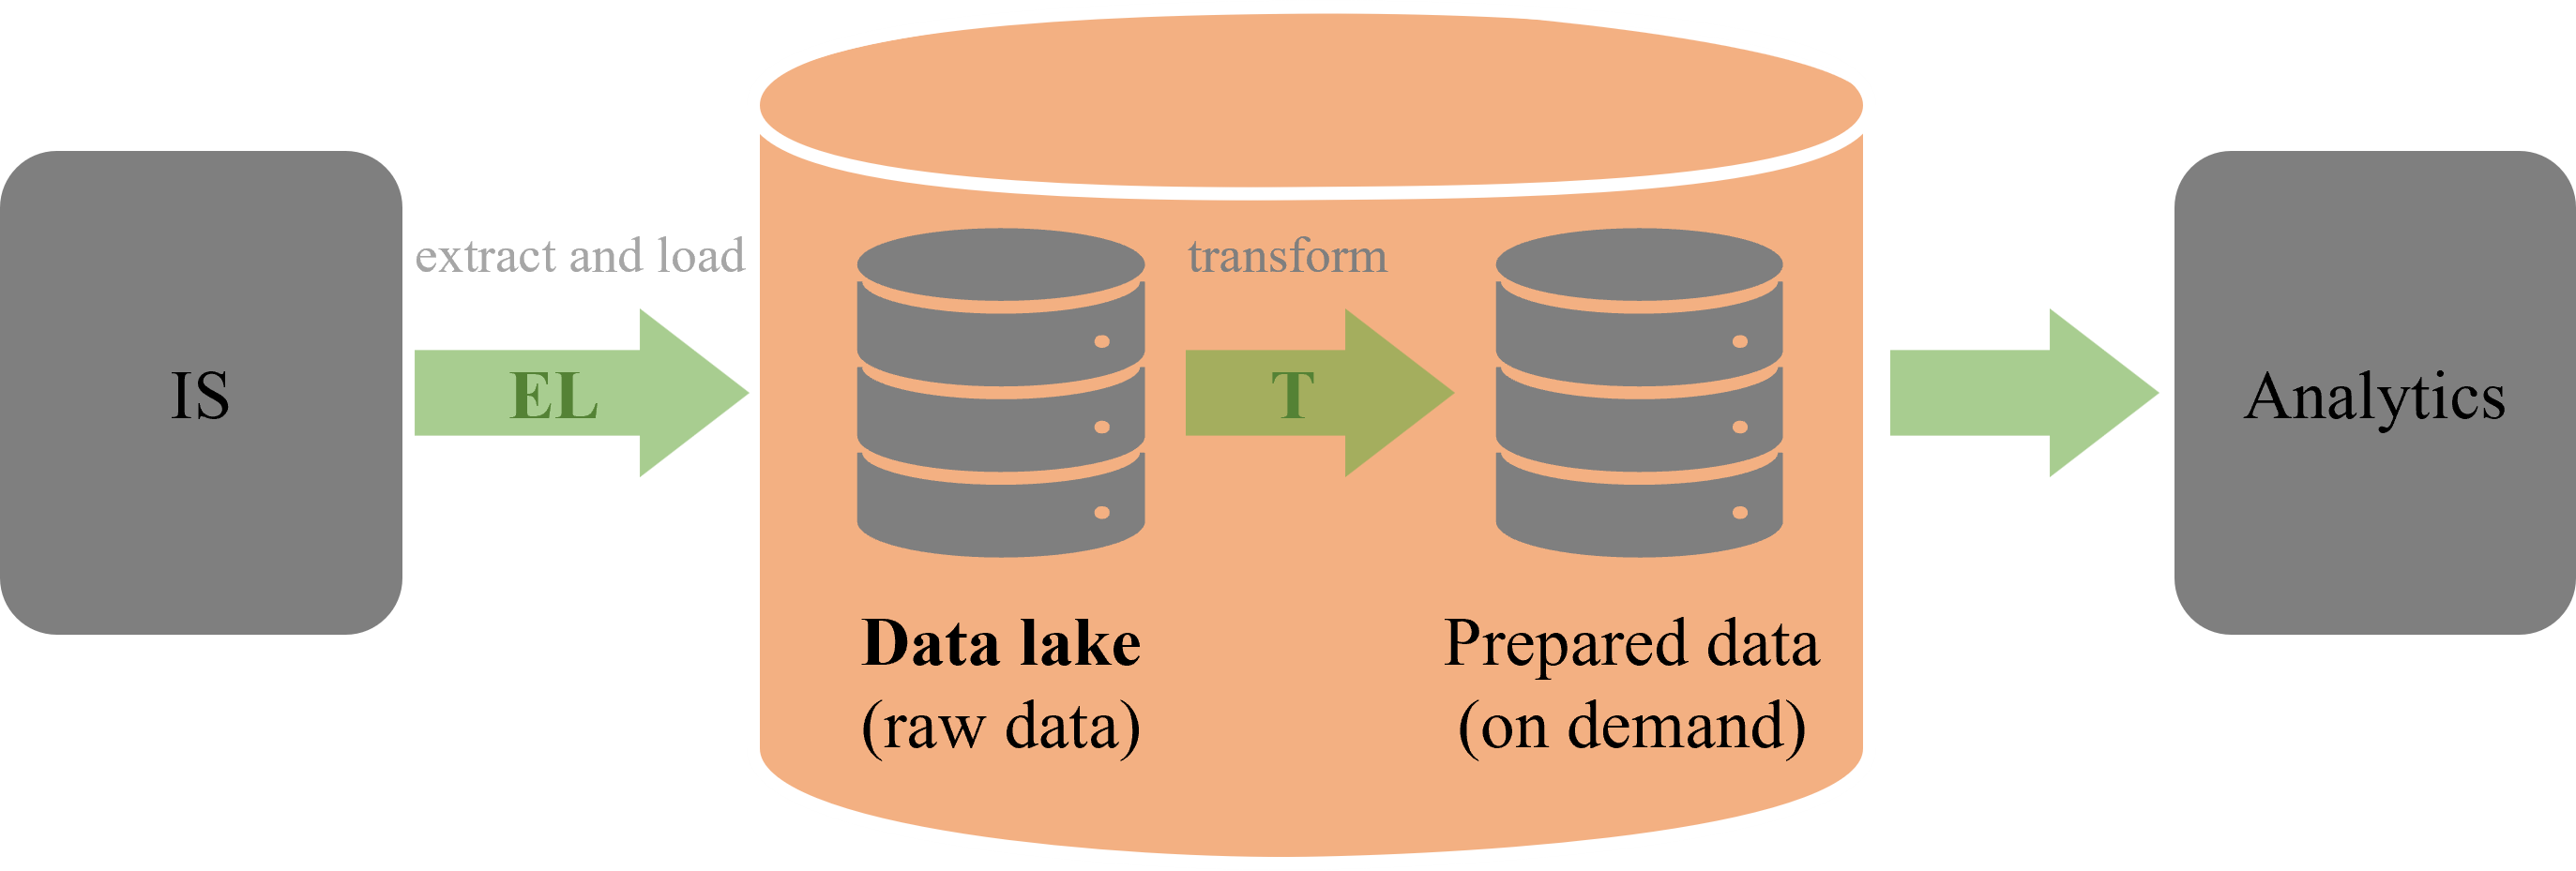
\includegraphics[width=0.45\textwidth]{assets/basics/elt.png}
  }

  \caption{Processes with extraction, transform, and load steps}
  \label{fig:1_etl_and_elt}
\end{figure}

As a final note on which steps are usually the most time-expensive: there is a so-called "80/20 rule" stating:
\begin{itemize}
  \item 80\% of a data scientist's time is spent on finding, cleaning, preprocessing, and organizing data. This leaves only 20\% to actually perform an analysis.
  \item On the other hand, we have 20\% effort determining 80\% of the final result.
\end{itemize}

\begin{figure}[H]
  \centering
  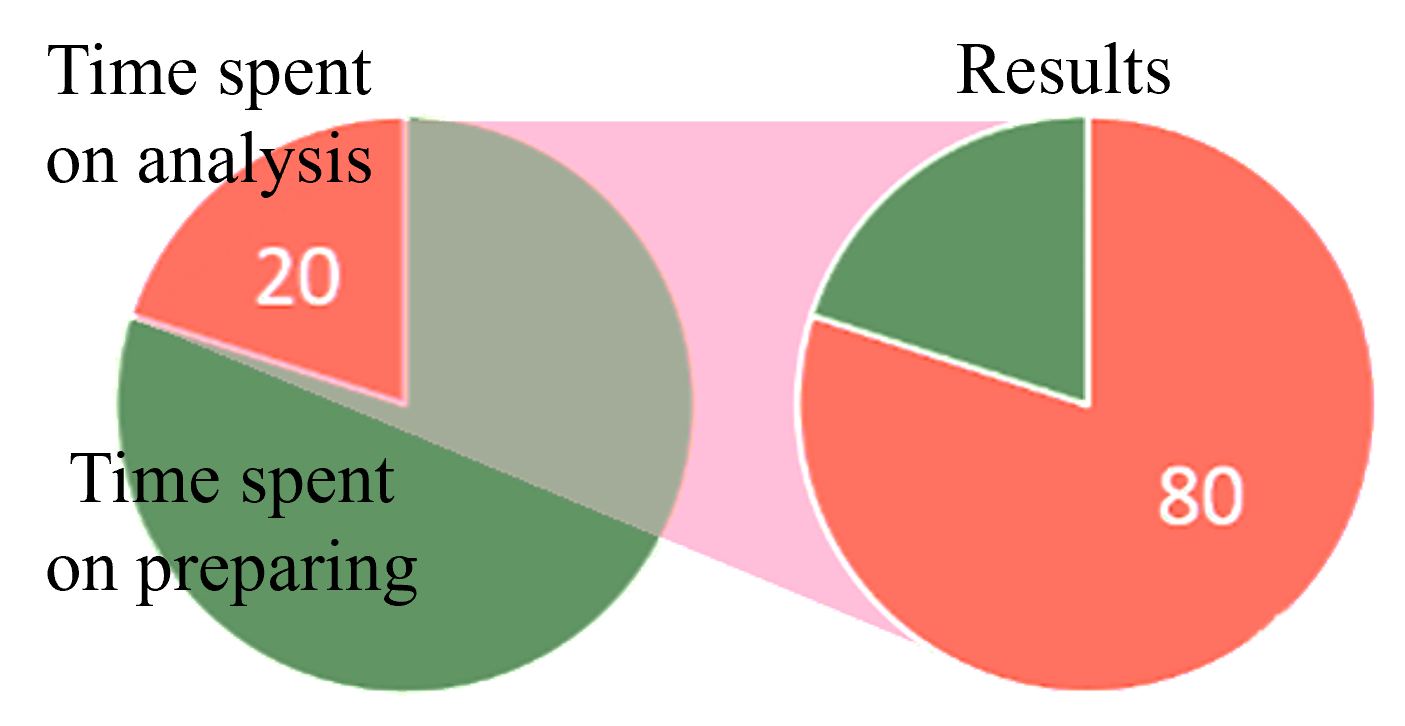
\includegraphics[width=0.4\textwidth]{assets/basics/80_20.png}
  \caption{80-20 rule}
  \label{fig:1_80_20}
\end{figure}
\subsection{Challenges}
To finalize the overview and basics of data science, let's look at the typical challenges.

First, we have the challenge of \textbf{finding data}. There may be hundreds or thousands of tables, for example in the case of SAP the numbers can easily for up to $800'000$. But, different entities differ in their relevance, meaning some are less relevant than others.

The next challenge is the \textbf{transformation of data}, meaning reorganization of data, filtering, extraction of relevant features, and so on. Not only for transformations, but also in general other challenges are \textbf{dealing with big data and streaming data}. The challenge of big data evolved over the last few decades, meaning typical stochastic methods try to solve the problem of saying something about entities given only a small amount of samples, whereas now we have a very high load of data, and need to solve the problem of dealing with these large amounts in a correct way. Also for streaming data, new approaches need to be thought of. Additionally, we also need to \textbf{deal with a concept shift}.

Another huge challenge is ensuring \textbf{data quality}. This goes especially, since our provided data may be incomplete, invalid, inconsistent, imprecise, and/or outdated. Consider for example timestamps. They might be 
\begin{itemize}
  \item Incomplete {\color{gray}\footnotesize(event is missing)}, 
  \item Invalid {\color{gray}\footnotesize(e.g. 14-14-2018)},
  \item Inconsistent {\color{gray}\footnotesize(14-07-2018 in contrast to 7-14-2018)}, or
  \item Imprecise {\color{gray}\footnotesize(only regard part of available data: 2018-09-21\textit{\st{'T'13:00:10}})}.
\end{itemize}

A very typical problem is \textbf{overfitting and underfitting} as it can be seen \ref{fig:1_over_under_fitting}.

\begin{figure}[H]
  \centering
  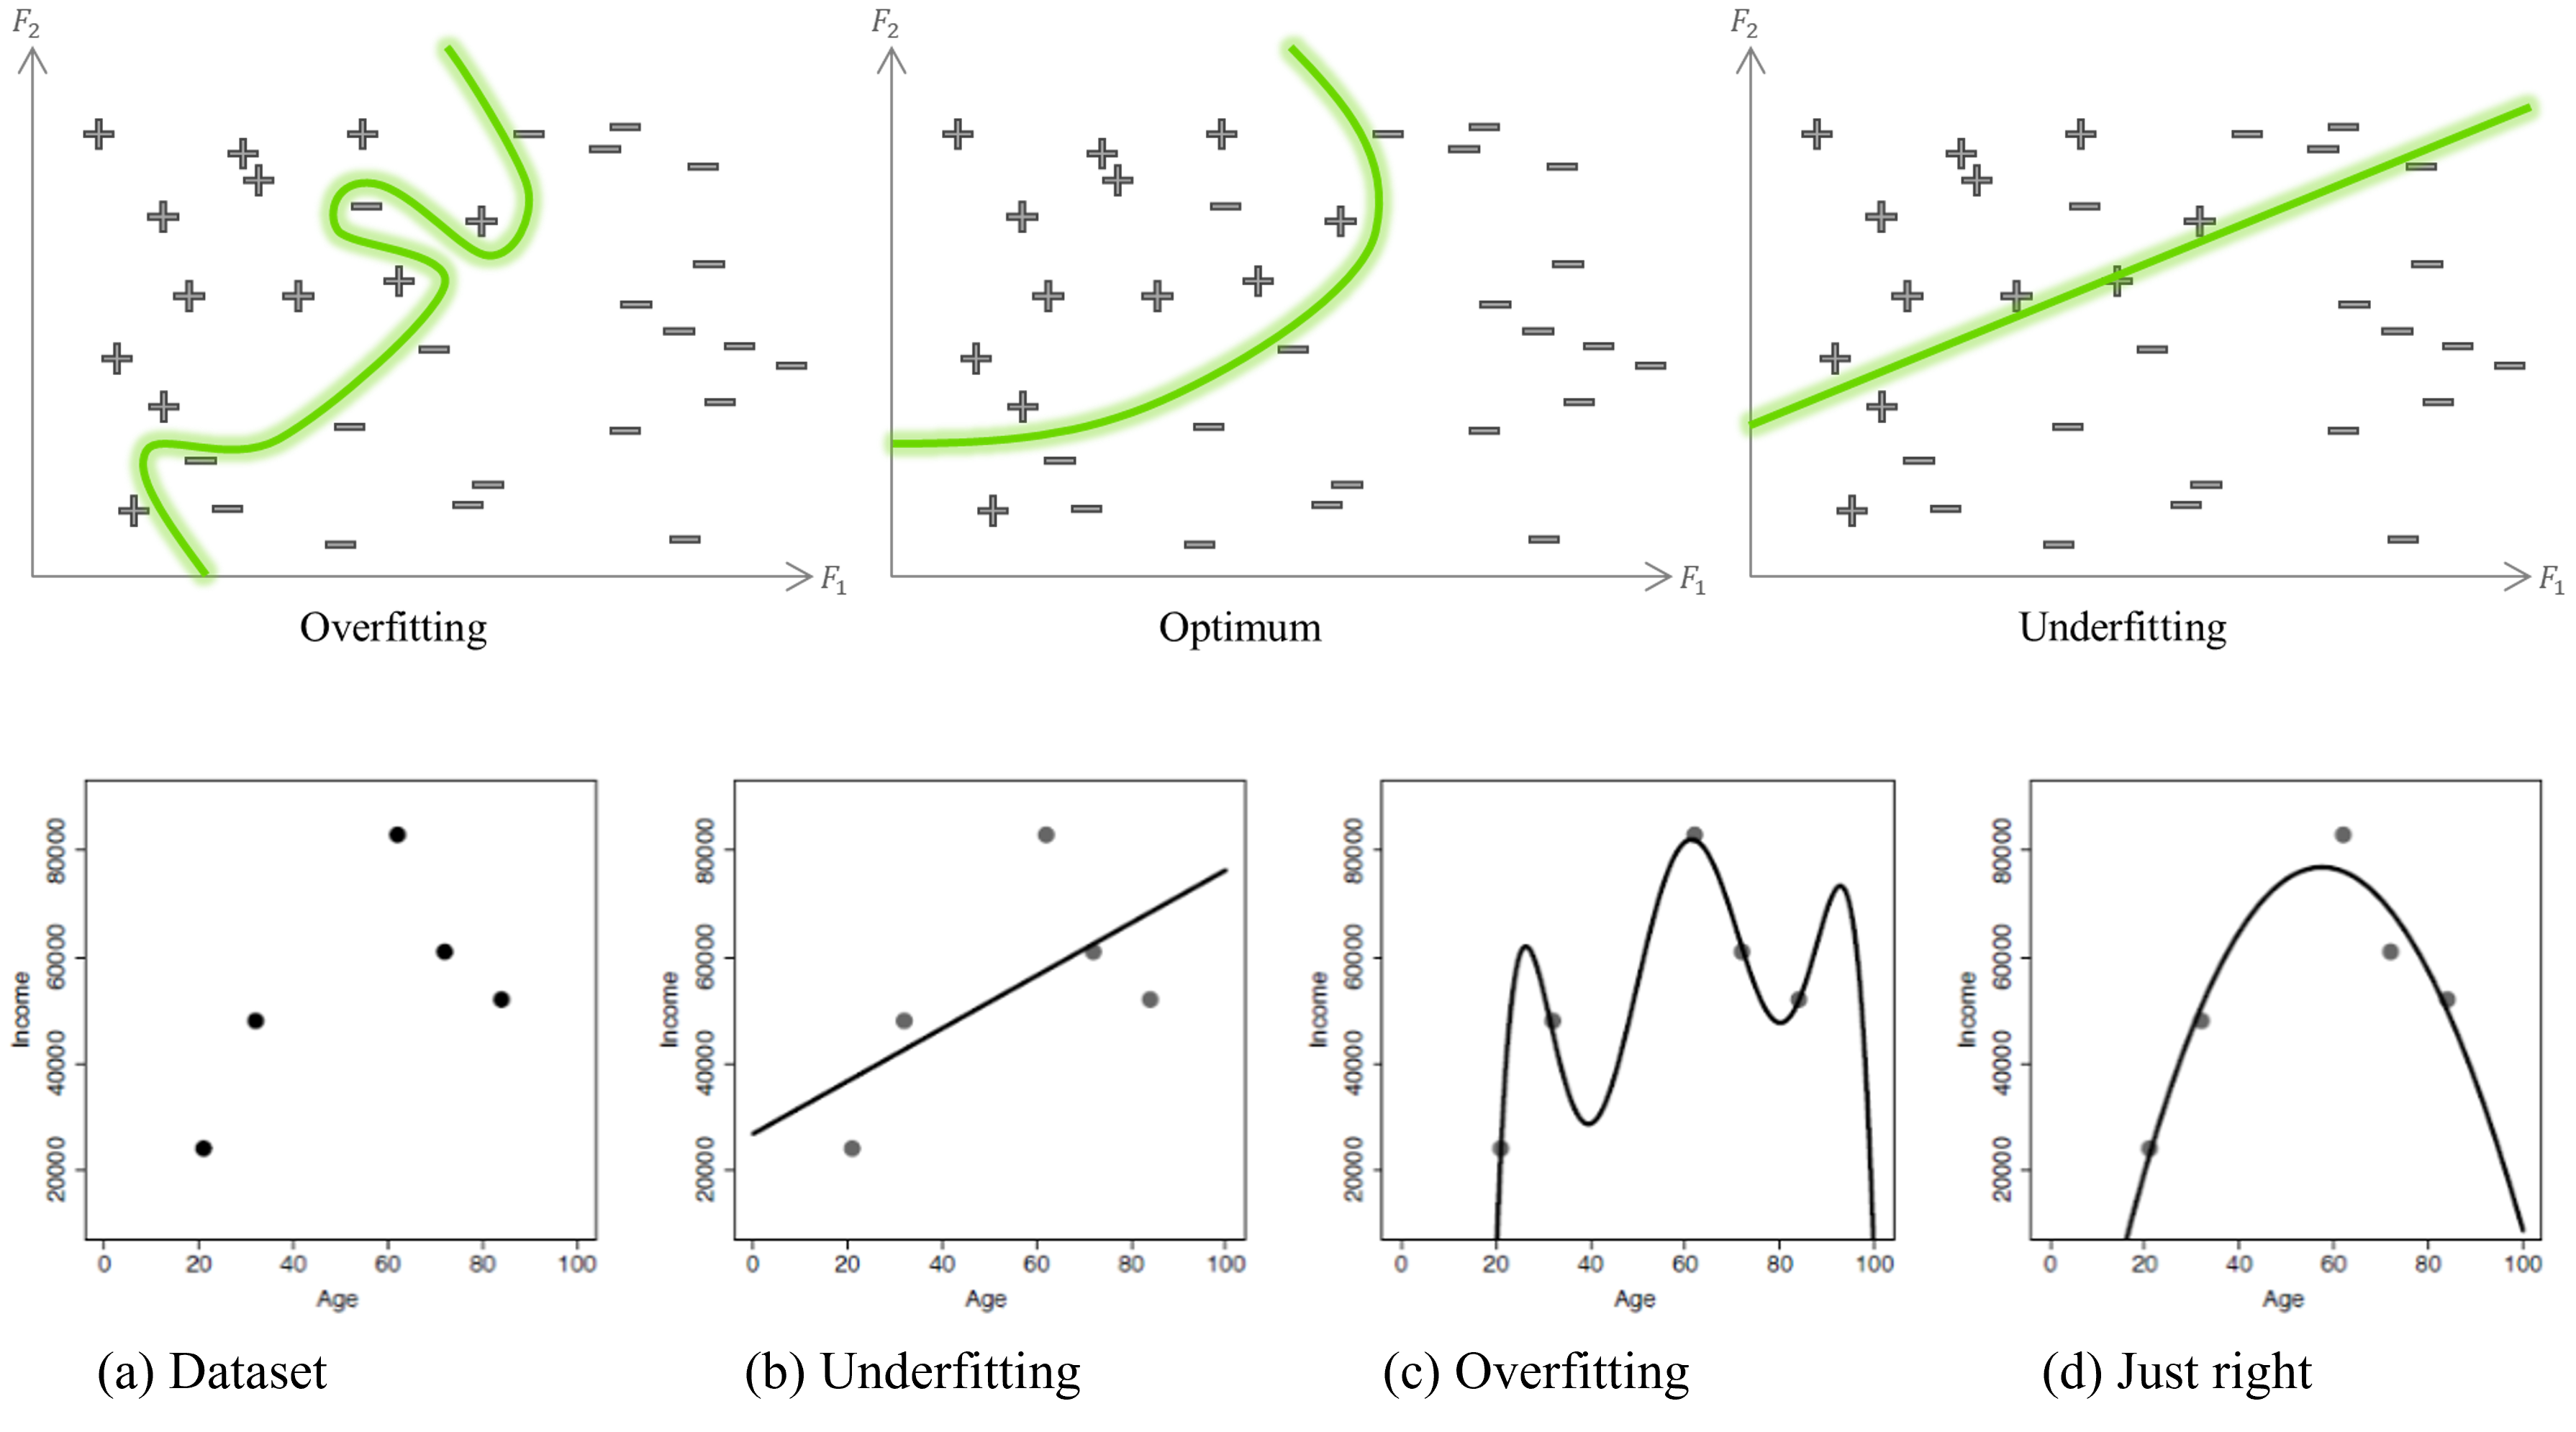
\includegraphics[width=0.9\textwidth]{assets/basics/over_under_fitting.png}
  \caption{Over- and underfitting visualized}
  \label{fig:1_over_under_fitting}
\end{figure}

The next challenge is the distinction of \textbf{correlation and causation}, explicitly that correlation does not imply causation. Consider this example:
\begin{itemize}
  \item Sunburn and ice cream have a strong correlation. When only these two features are considered, one might derive that either ice cream causes sunburn, or the other way around.
  \item We know of course, that this is not correct and instead an additional factor causes both phenomena: if the sun is shining, it's warm and people eat ice cream, and also sun directly causes sunburn.
\end{itemize}

Besides the accuracy of our results, we also need to look into whether our results are valuable. Concretely, \textbf{results} should be \textbf{made actionable}. This means, that analysis results should be relevant, specific, timely, novel, and clear. Our goal is to go from "data" to "insight" and finally "action". Consider these examples:
\begin{itemize}
  \item Warning about a traffic jam should come before entering said traffic jam.
  \item That it's currently raining is not too helpful information. Preferably is a notice ahead of time.
\end{itemize}

The last, but very important challenge is \textbf{responsible data science} (RDS)\sidenote{Responsible data science}. This includes ensuring of:
\begin{itemize}
  \item \textbf{Fairness}, meaning data science should exclude prejudice {\color{gray}\footnotesize(How to avoid unfair conclusions even if they are true?)}
  \item \textbf{Accuracy}, so data science without guesswork {\color{gray}\footnotesize(How to answer questions with a guaranteed level of accuracy?)}
  \item \textbf{Confidentiality} {\color{gray}\footnotesize(How to answer questions without revealing secrets?)}
  \item \textbf{Transparency} {\color{gray}\footnotesize(How to clarify answers such that they become indisputable?)}
\end{itemize}
